\chapter{Verified Diff Array Implementation}\label{chapter:diff-array}
 
In the following, we will implement and verify diff arrays using Imperative/HOL (\autoref{section:imperative_hol}) and separation logic (\autoref{section:separation-logic-hol}) facilities.
 
\section{Cell}

As the base building block for our diff array implementation, we use a sum type called |cell| (\autoref{fig:cell_type}).

\begin{figure}[htpb]
    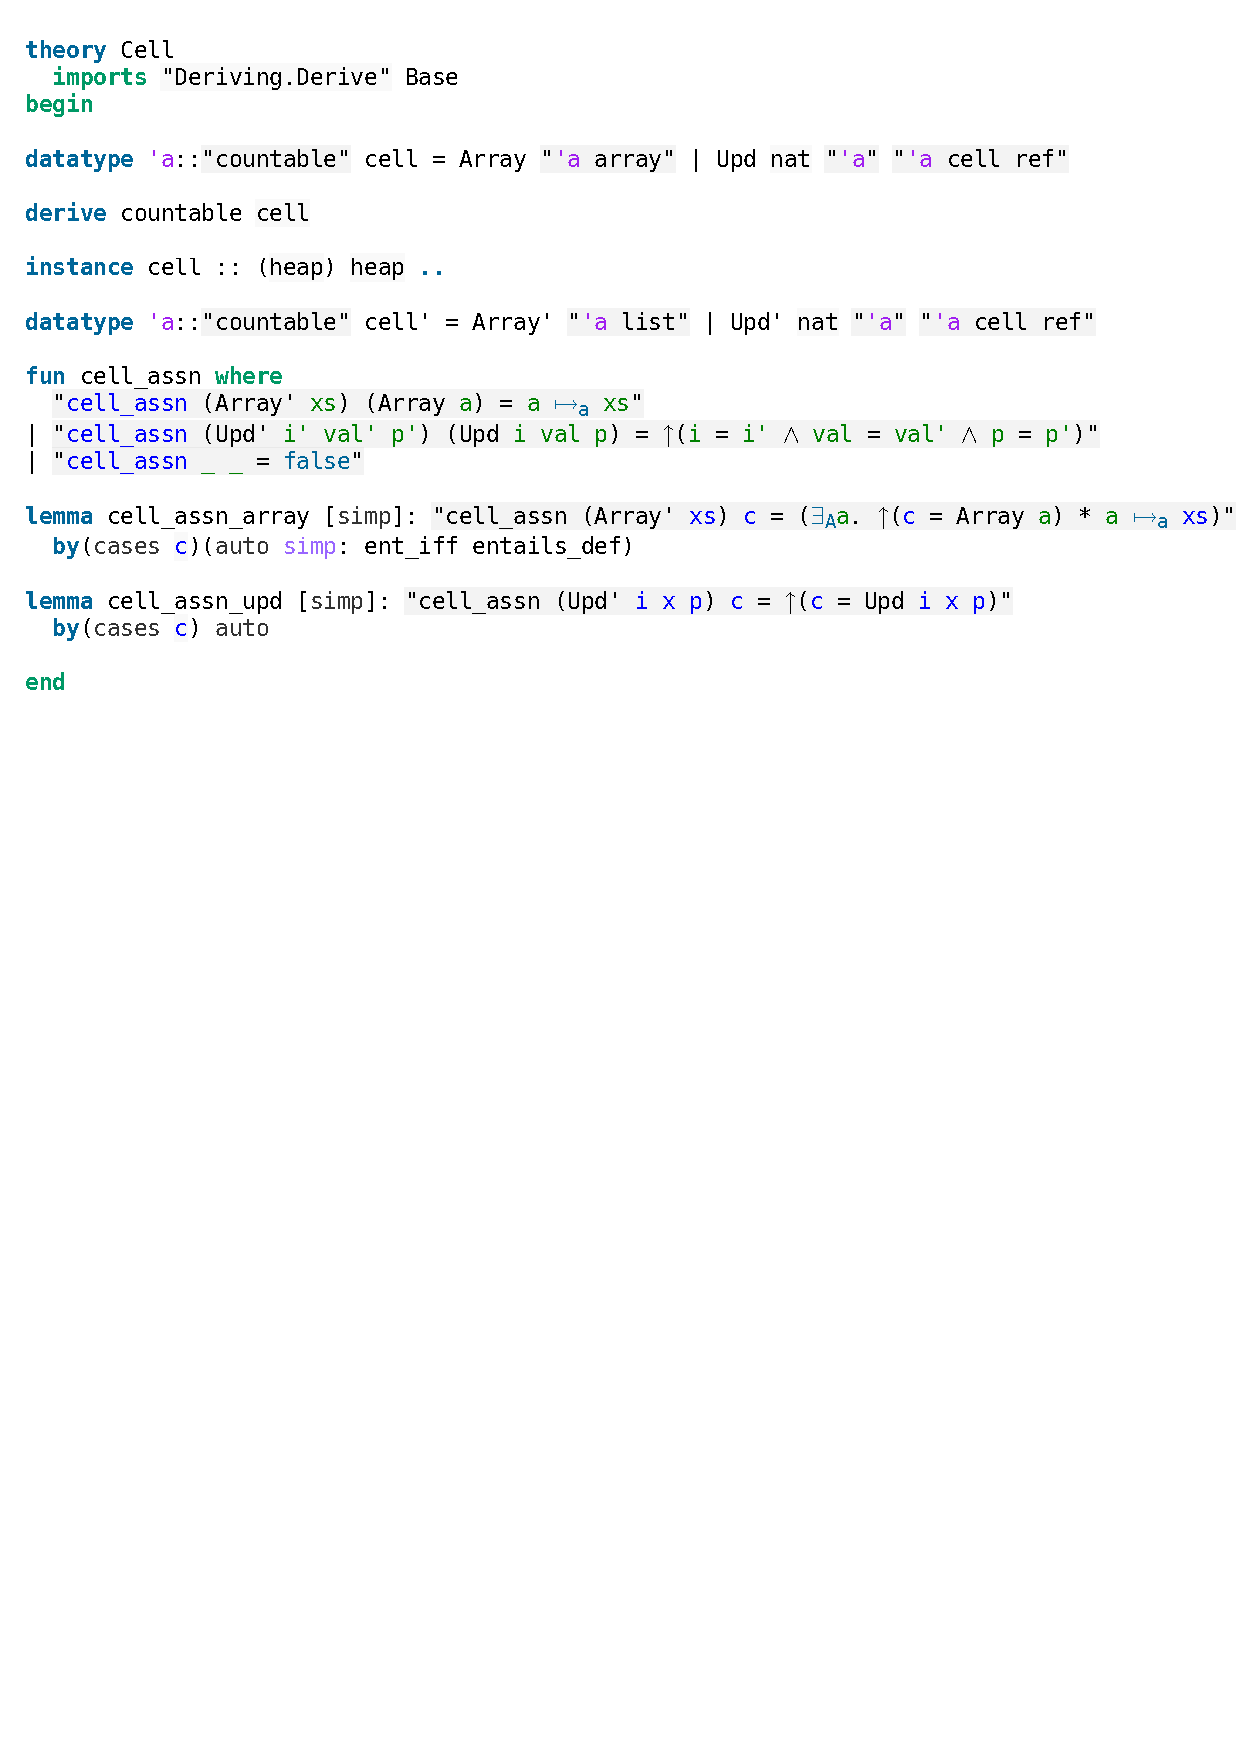
\includegraphics[trim={0 26,7cm 0 2,5cm}, clip, width=1.00\textwidth]{figures/Theory_Cell.pdf}
    \caption[Cell type]{Cell type}
    \label{fig:cell_type}
\end{figure}

\noindent It either directly contains an array or an update at a specific index and a reference to another |cell| stored on the heap. The type of the |cell|'s value must be |countable| because the heap can only store |countable| types. Through that, we can derive that |cell| as a whole is |countable| and satisfies the |heap| type class.
As an abstract representation of |cell|, we implement |cell|' (\autoref{fig:cell'_type}), which only differs from |cell| in that it stores a list instead of an array.

\begin{figure}[htpb]
    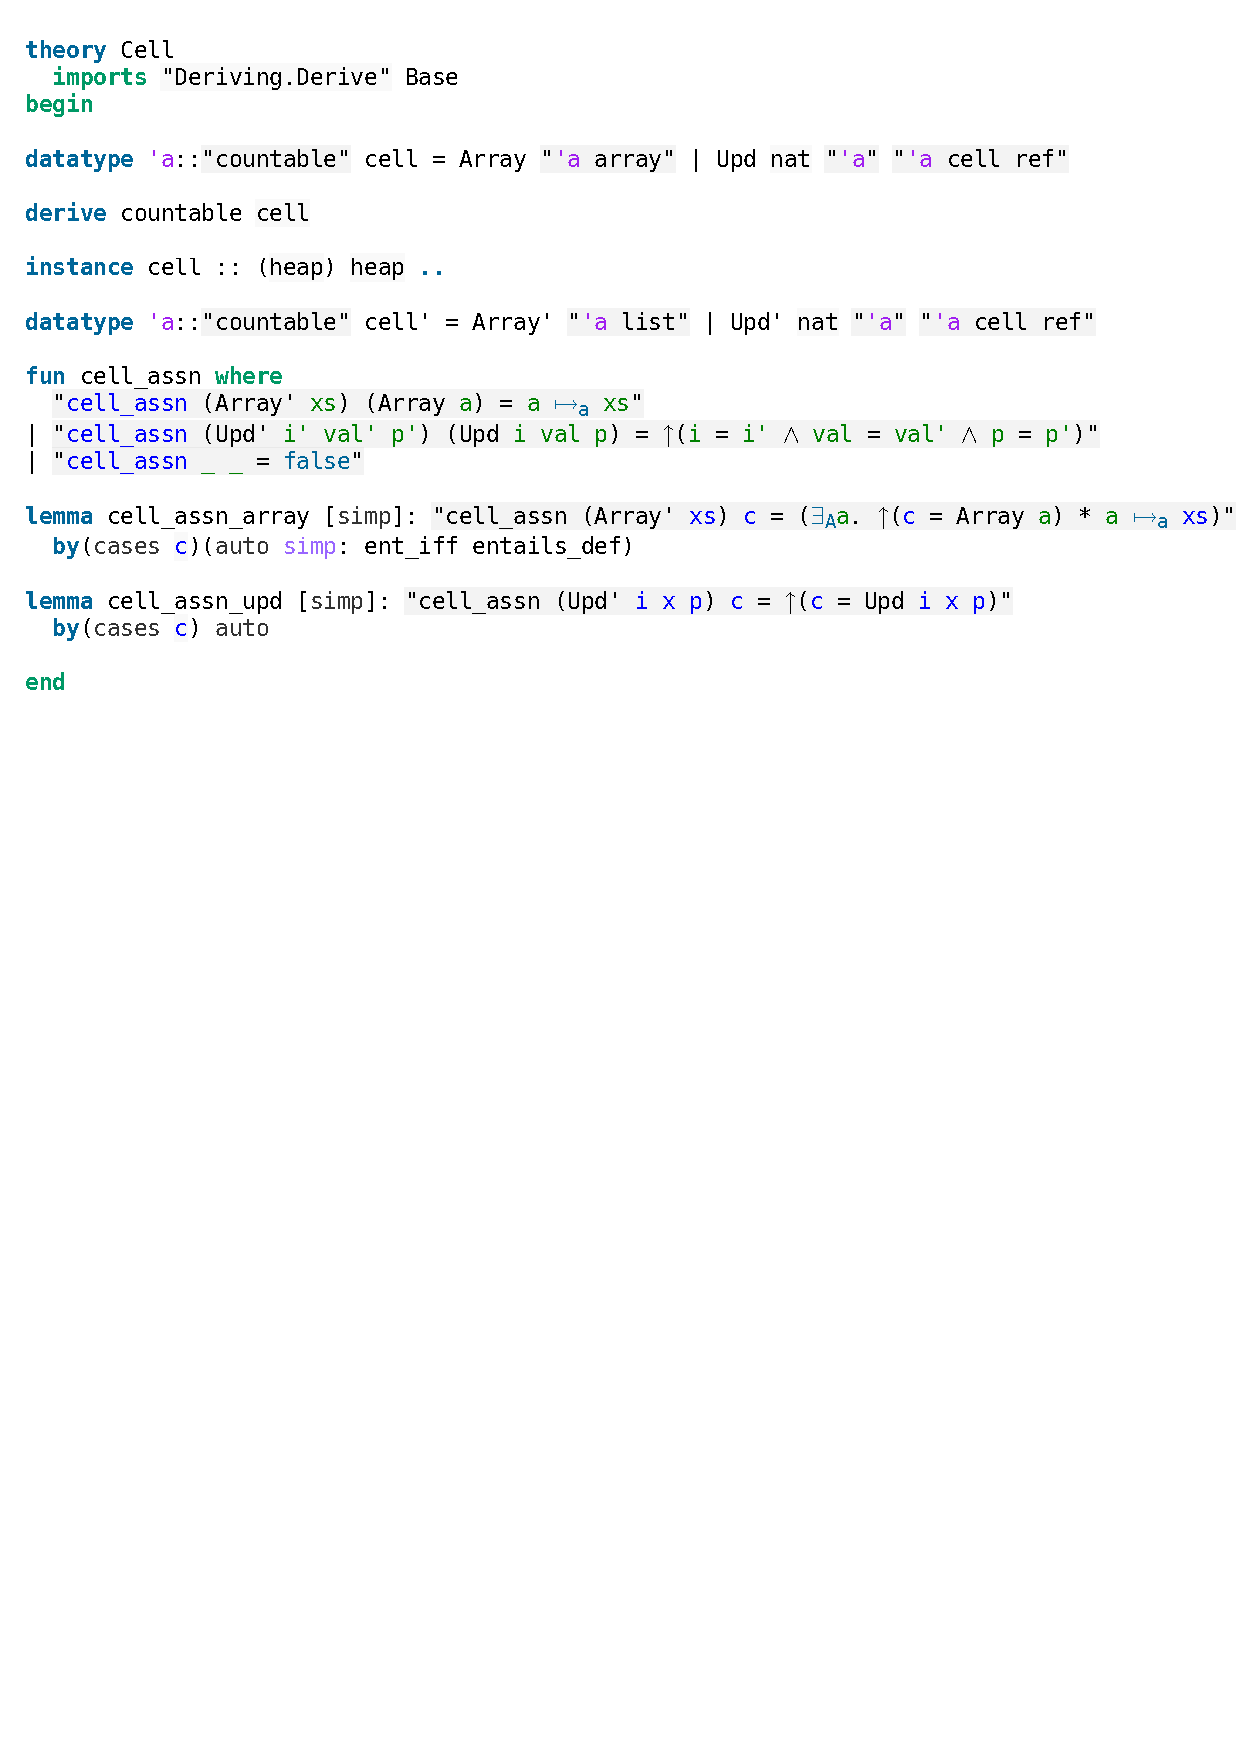
\includegraphics[trim={0 24cm 0 5cm}, clip, width=1.00\textwidth]{figures/Theory_Cell.pdf}
    \caption[Cell' type]{Cell' type}
    \label{fig:cell'_type}
\end{figure}

\noindent Using separation logic assertions, we use the cell assertion function in \autoref{fig:cell_assertion} to correspond cells with their abstractions.

\begin{figure}[htpb]
    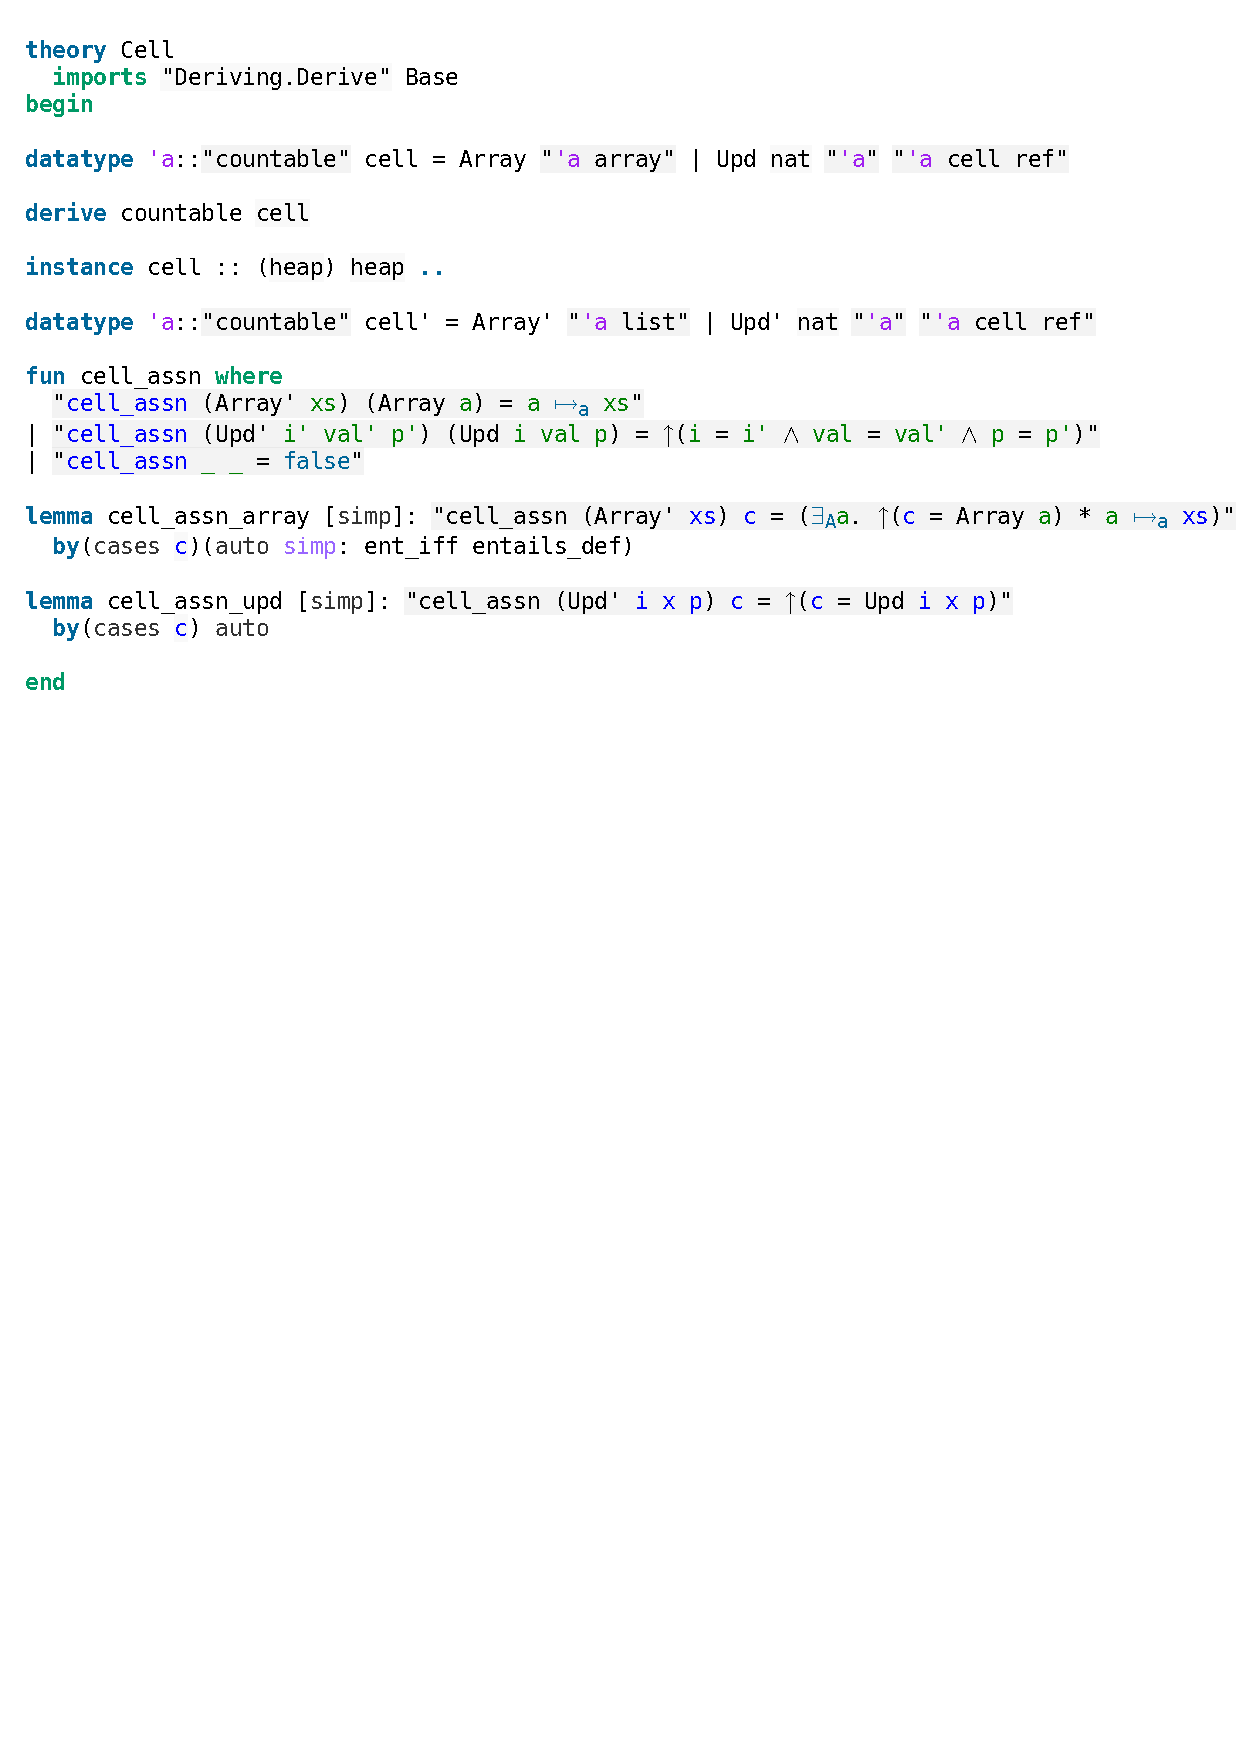
\includegraphics[trim={0 21,4cm 0 6,2cm}, clip, width=1.00\textwidth]{figures/Theory_Cell.pdf}
    \caption[Cell assertion]{Cell assertion}
    \label{fig:cell_assertion}
\end{figure}

\noindent The abstraction happens in the first case of the function, such that we assert that the array of |cell| points to the specified list in |cell|’, meaning that the array contains the same elements as the list. For the update cases, we simply assert that the index, value, and pointer are the same using a pure assertion. One would naturally think of recursing on the pointer here, but it is not possible due to how separation logic works: Since we can have multiple updates which point to the same array, we would recurse multiple times to the leaf node. It would result in separating multiple assertions representing the same pointer, which yields |false| in separation logic. We would restrict ourselves to one version per diff array, which defeats the purpose of diff arrays.

\section{Diff Array Relation}

We solve this issue by having references of all |cell|s of a diff array, and their corresponding |cell|'s in a list. Using this list, which we will mostly call |t|, we can assert the structure of the diff arrays using a pure assertion, meaning standard boolean logic. We create the relation (\autoref{fig:diff_arr_rel'}) by recursing on the number of stored updates before reaching the actual array.

\begin{figure}[htpb]
    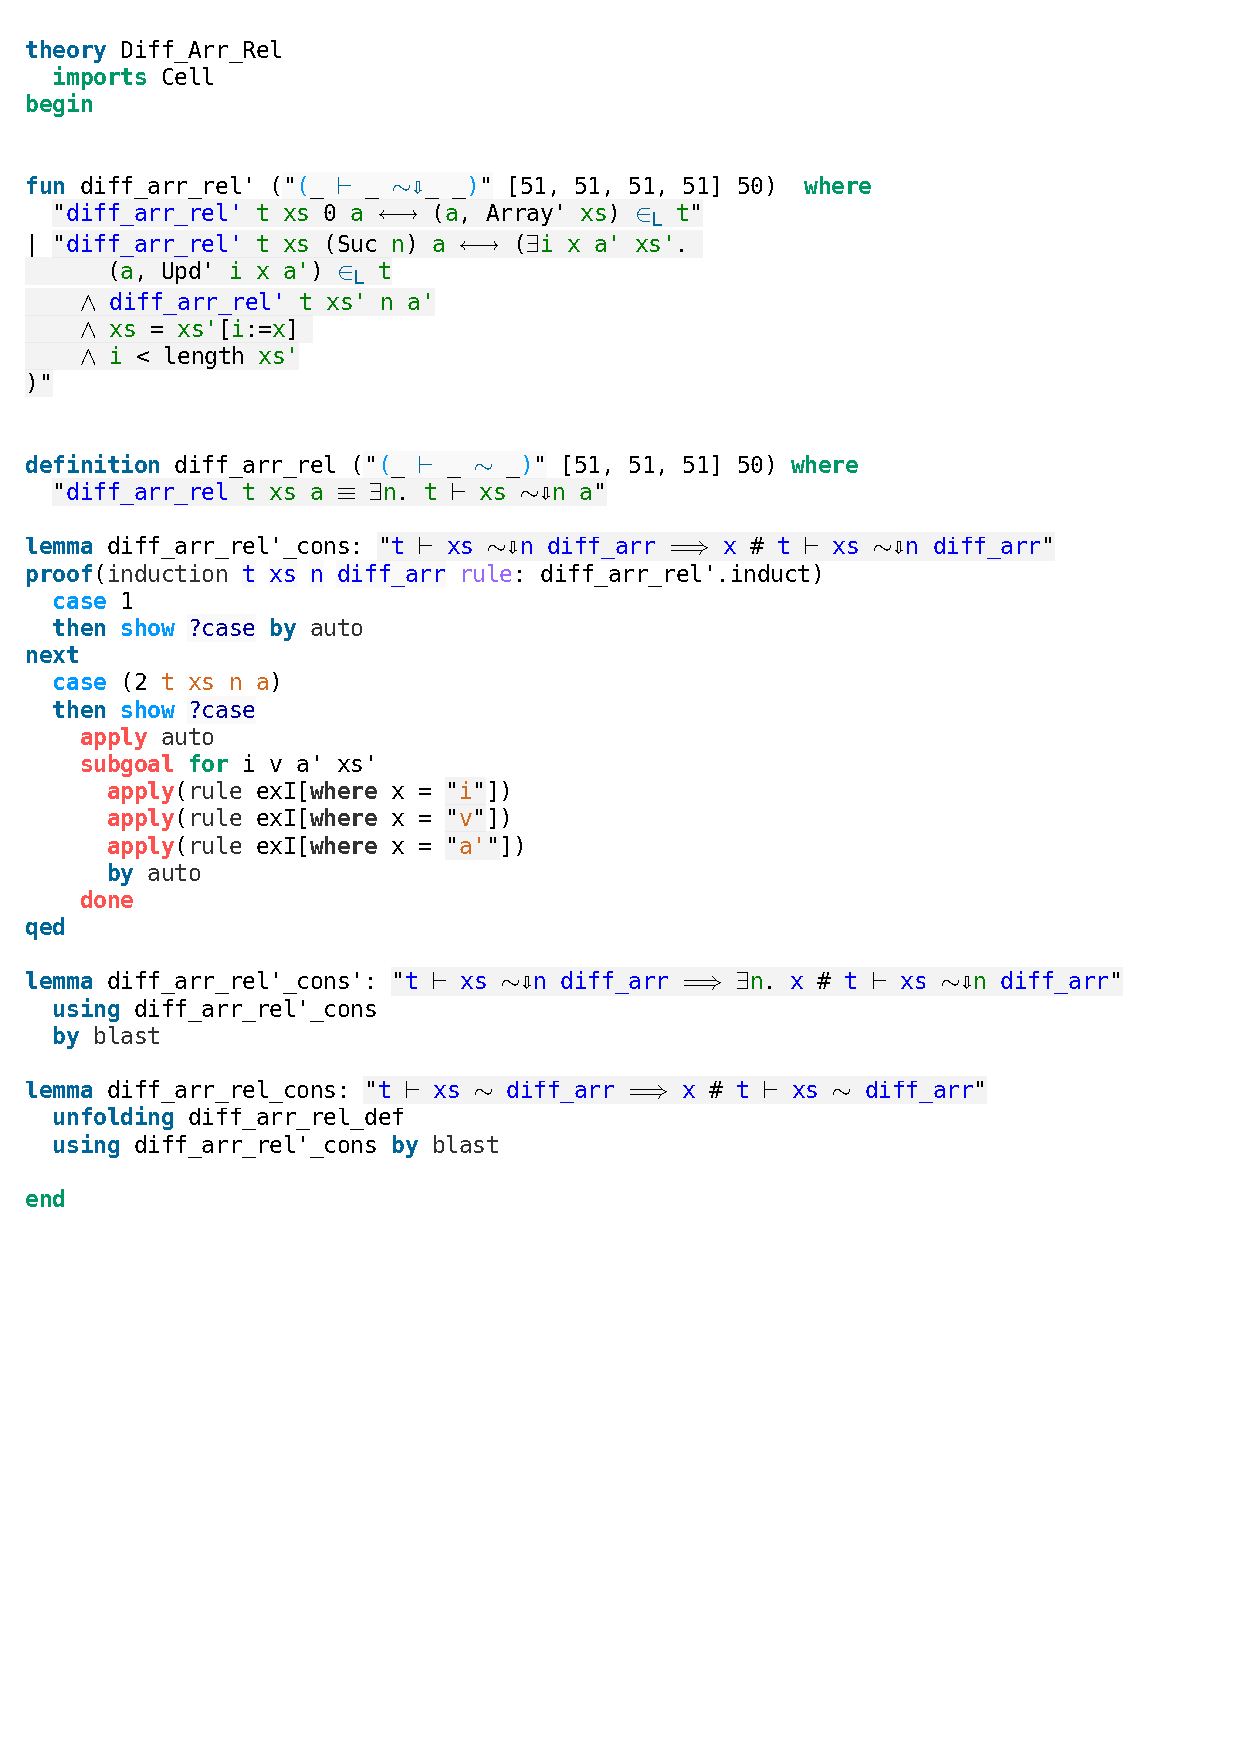
\includegraphics[trim={0 22,4cm 0 2,9cm}, clip, width=1.00\textwidth]{figures/Theory_Diff_Arr_Rel.pdf}
    \caption[Diff array relation]{Diff array relation\footnotemark}
    \label{fig:diff_arr_rel'}
\end{figure}
\footnotetext{$x$ $\in_L$ $xs$ is a short-hand notation for $x$ $\in$ $set$ $xs$}

\noindent In the base case, when the number of updates is zero, we assert that |t| contains the abstract list representation and the |cell| reference. On the other hand, if the number of updates exceeds zero, we assume that the |cell| reference is in |t| together with an update entry. Furthermore, the index of the update needs to be in bounds of the list abstraction, and the whole relation needs to hold recursively for the reference in the update with the update reversely applied. As a short-hand notation for the diff array relation, we use $t$ $\vdash$ $xs$ $\sim_n$ $a$. In the following, we mostly will not care about the exact number of updates and existentially quantify it with the definition in \autoref{fig:diff_arr_rel} and its corresponding short-hand notation $t$ $\vdash$ $xs$ $\sim$ $a$.

\begin{figure}[htpb]
    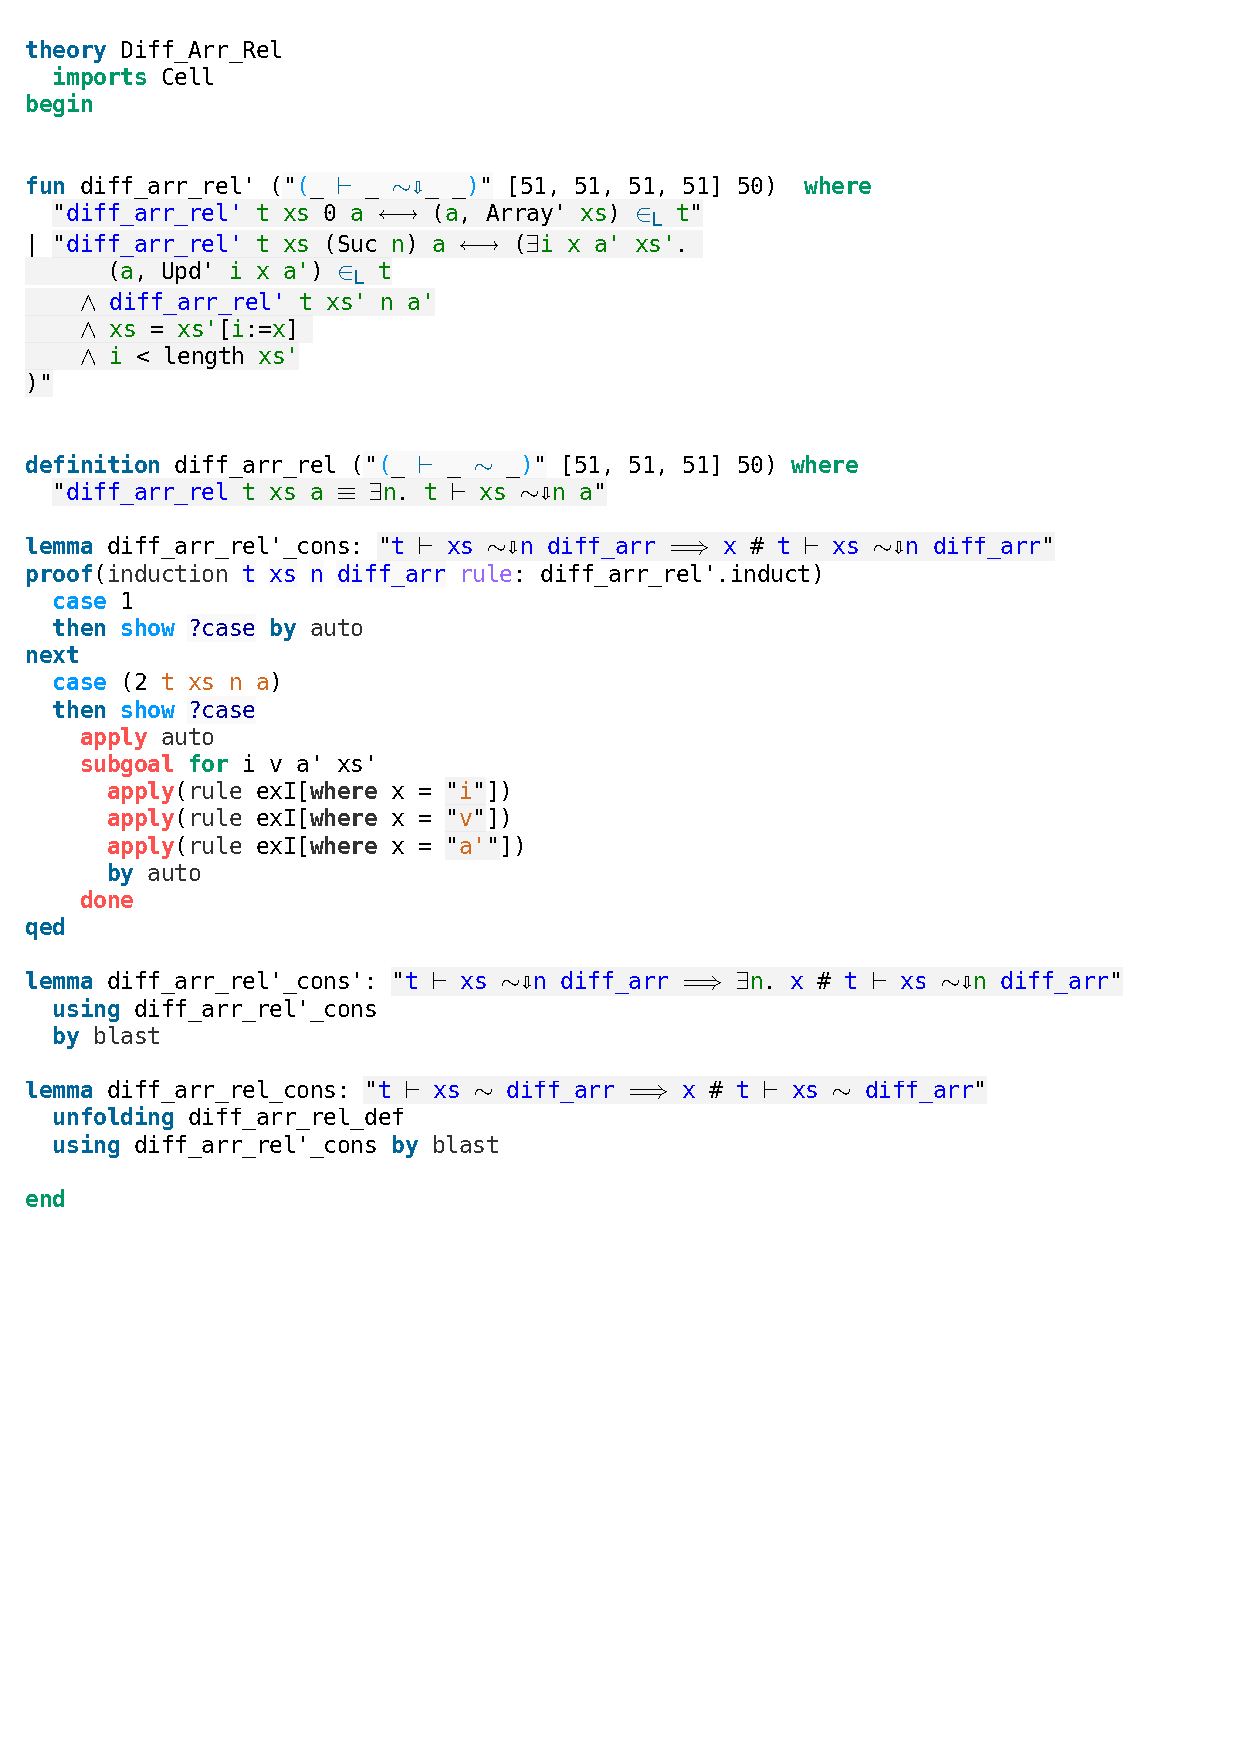
\includegraphics[trim={0 21,2cm 0 7,4cm}, clip, width=1.00\textwidth]{figures/Theory_Diff_Arr_Rel.pdf}
    \caption[Existentially quantified diff array relation]{Existentially quantified diff array relation}
    \label{fig:diff_arr_rel}
\end{figure}

\noindent A straightforward property we can prove at this point is that we can add arbitrary elements to the list |t| without interfering with the relation (\autoref{fig:diff_arr_rel_cons}).

\begin{figure}[htpb]
    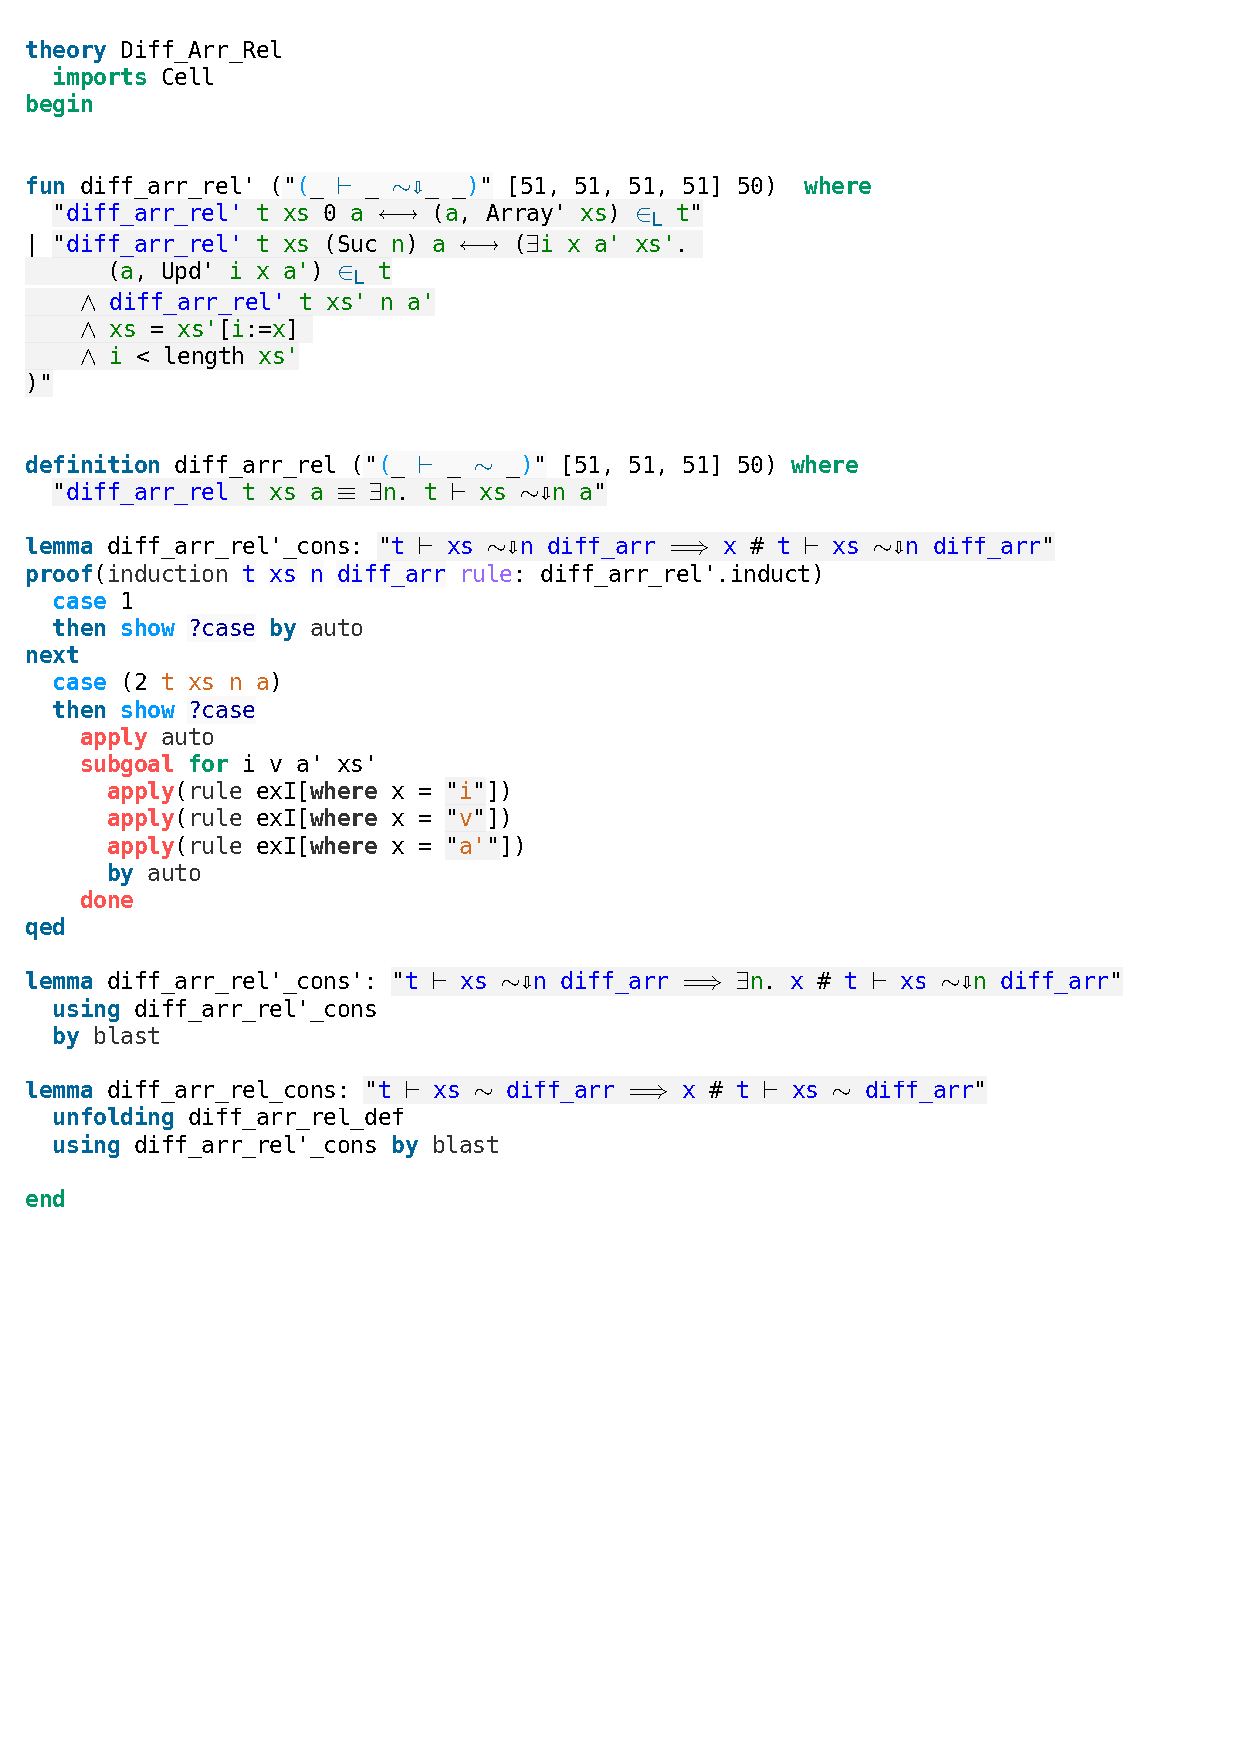
\includegraphics[trim={0 11cm 0 18,2cm}, clip, width=1.00\textwidth]{figures/Theory_Diff_Arr_Rel.pdf}
    \caption[Add element to diff array relation]{Adding an element to a diff array relation does not interfere with it}
    \label{fig:diff_arr_rel_cons}
\end{figure}

\section{Master Assertion}\label{section:master_assn}

To build the bridge between the list on which the diff array relation is working and the cell assertions, we define a master assertion (\autoref{fig:master_assn}). 

\begin{figure}[htpb]
    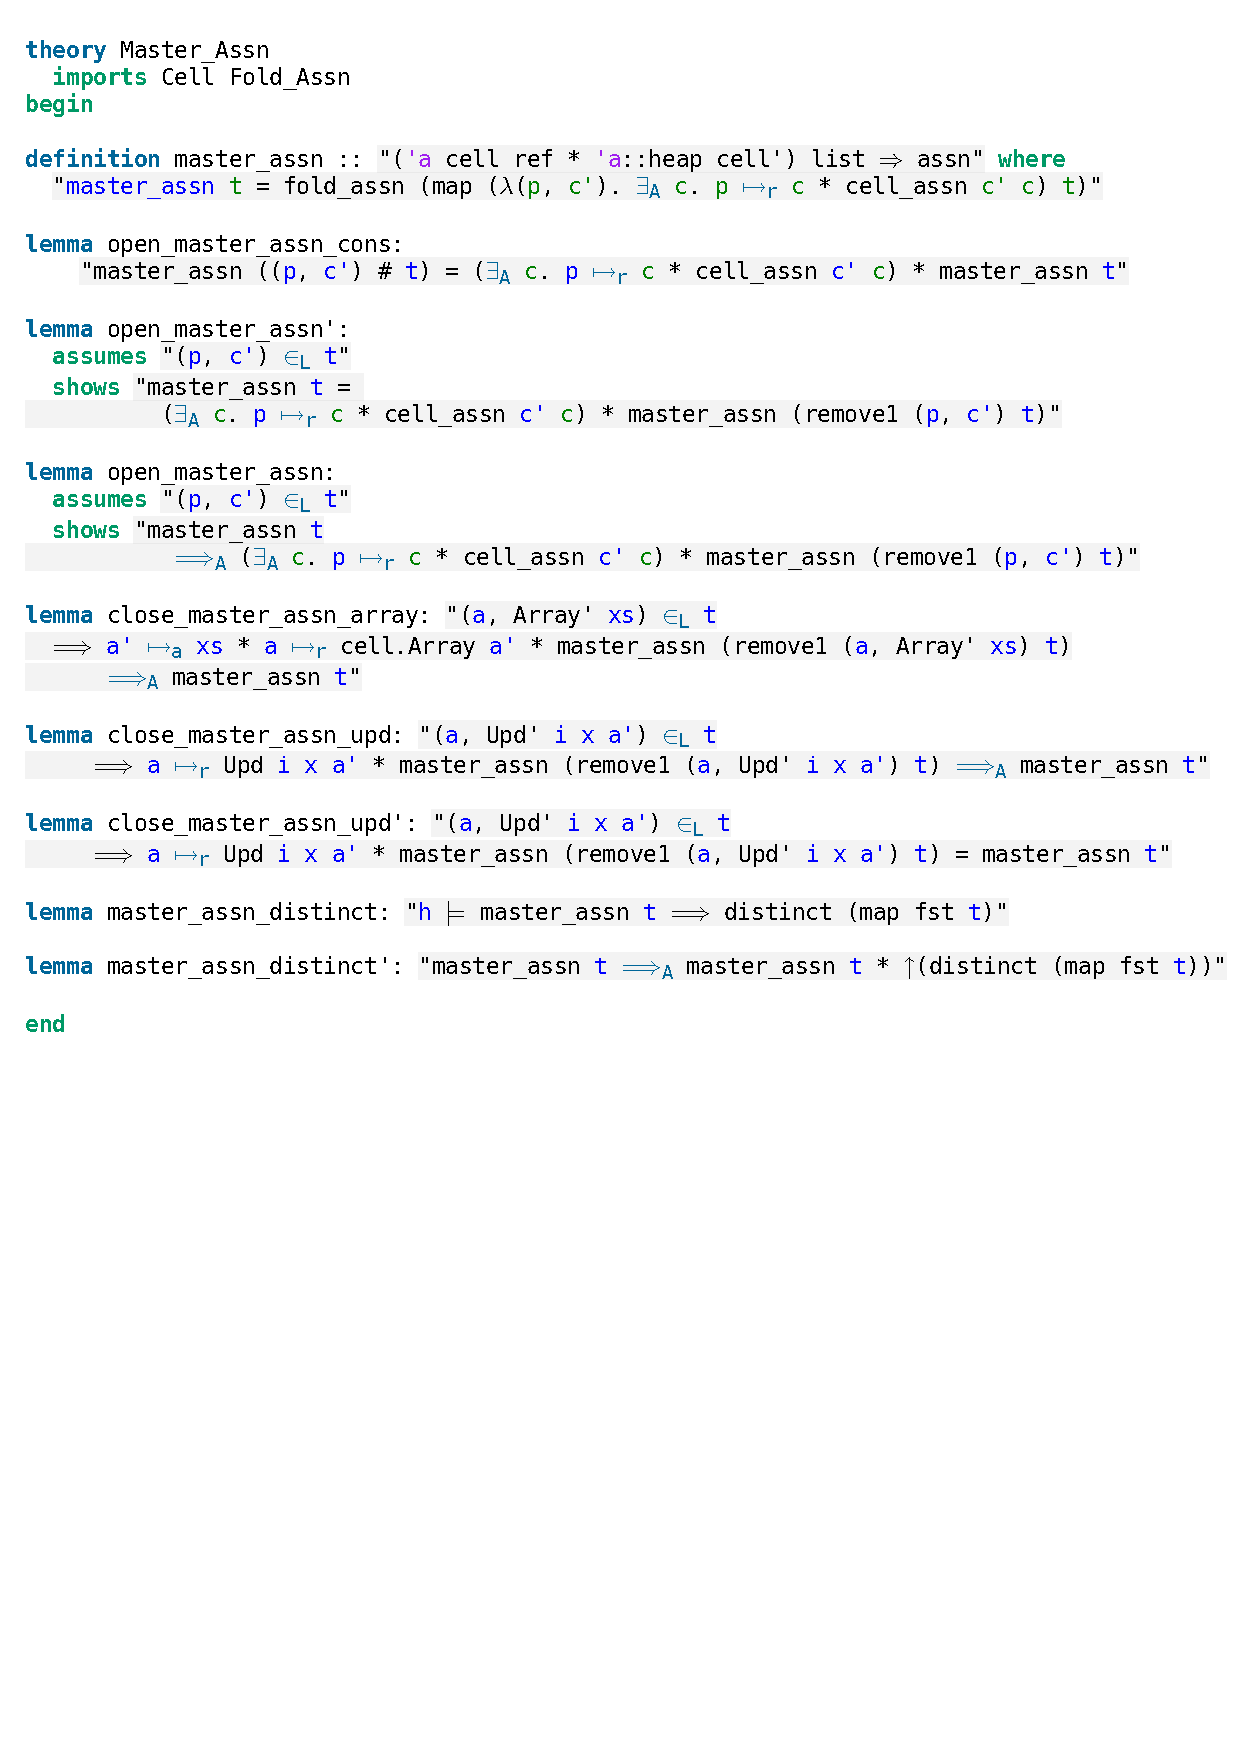
\includegraphics[trim={0 26,3cm 0 2cm}, clip, width=1.00\textwidth]{figures/Theory_Master_Assn.pdf}
    \caption[Master assertion]{Master assertion}
    \label{fig:master_assn}
\end{figure}

\noindent For that, we map |t| to assertions by firstly dereferencing the |cell|s using existential quantification in separation logic and the |points-to| relation for references. Secondly, we relate this |cell| with the corresponding |cell|’ using the cell assertion.
In the next step, we fold the assertions using the separation conjunction. The implementation of this |fold| is straightforward and uses the empty assertion as the start value (\autoref{fig:fold_assn}).

\begin{figure}[htpb]
    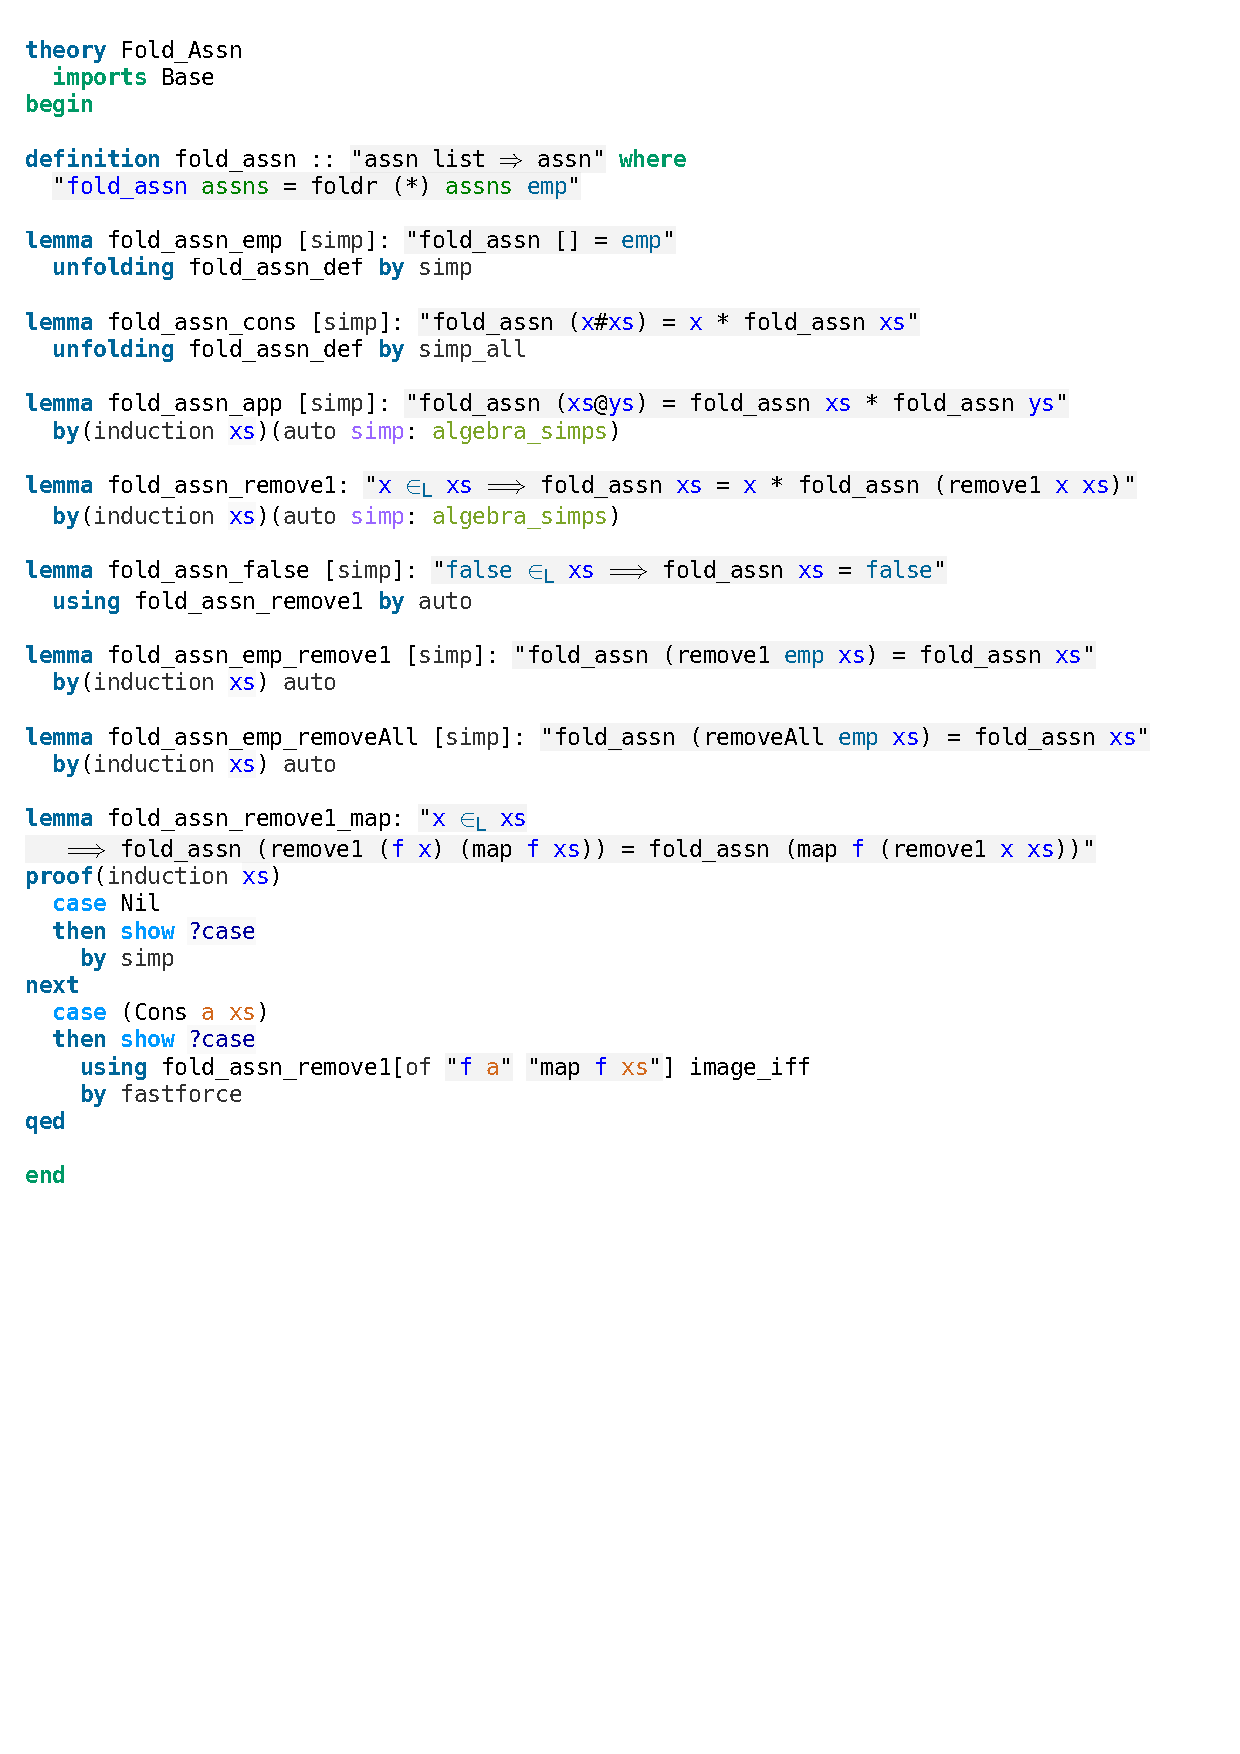
\includegraphics[trim={0 26,3cm 0 2,3cm}, clip, width=1.00\textwidth]{figures/Theory_Fold_Assn.pdf}
    \caption[Fold assertions]{Fold assertions}
    \label{fig:fold_assn}
\end{figure}

\noindent We show some basic properties of this fold to make the reasoning over the master assertion easier. They do not yield surprises but let us create some useful lemmas for "opening" and "closing" master assertions (\autoref{fig:master_assn_lemmas}).\footnote{With "open", we mean extracting an element from the master assertion, and with "close", adding an element to the master assertion.}

\begin{figure}[htpb]
    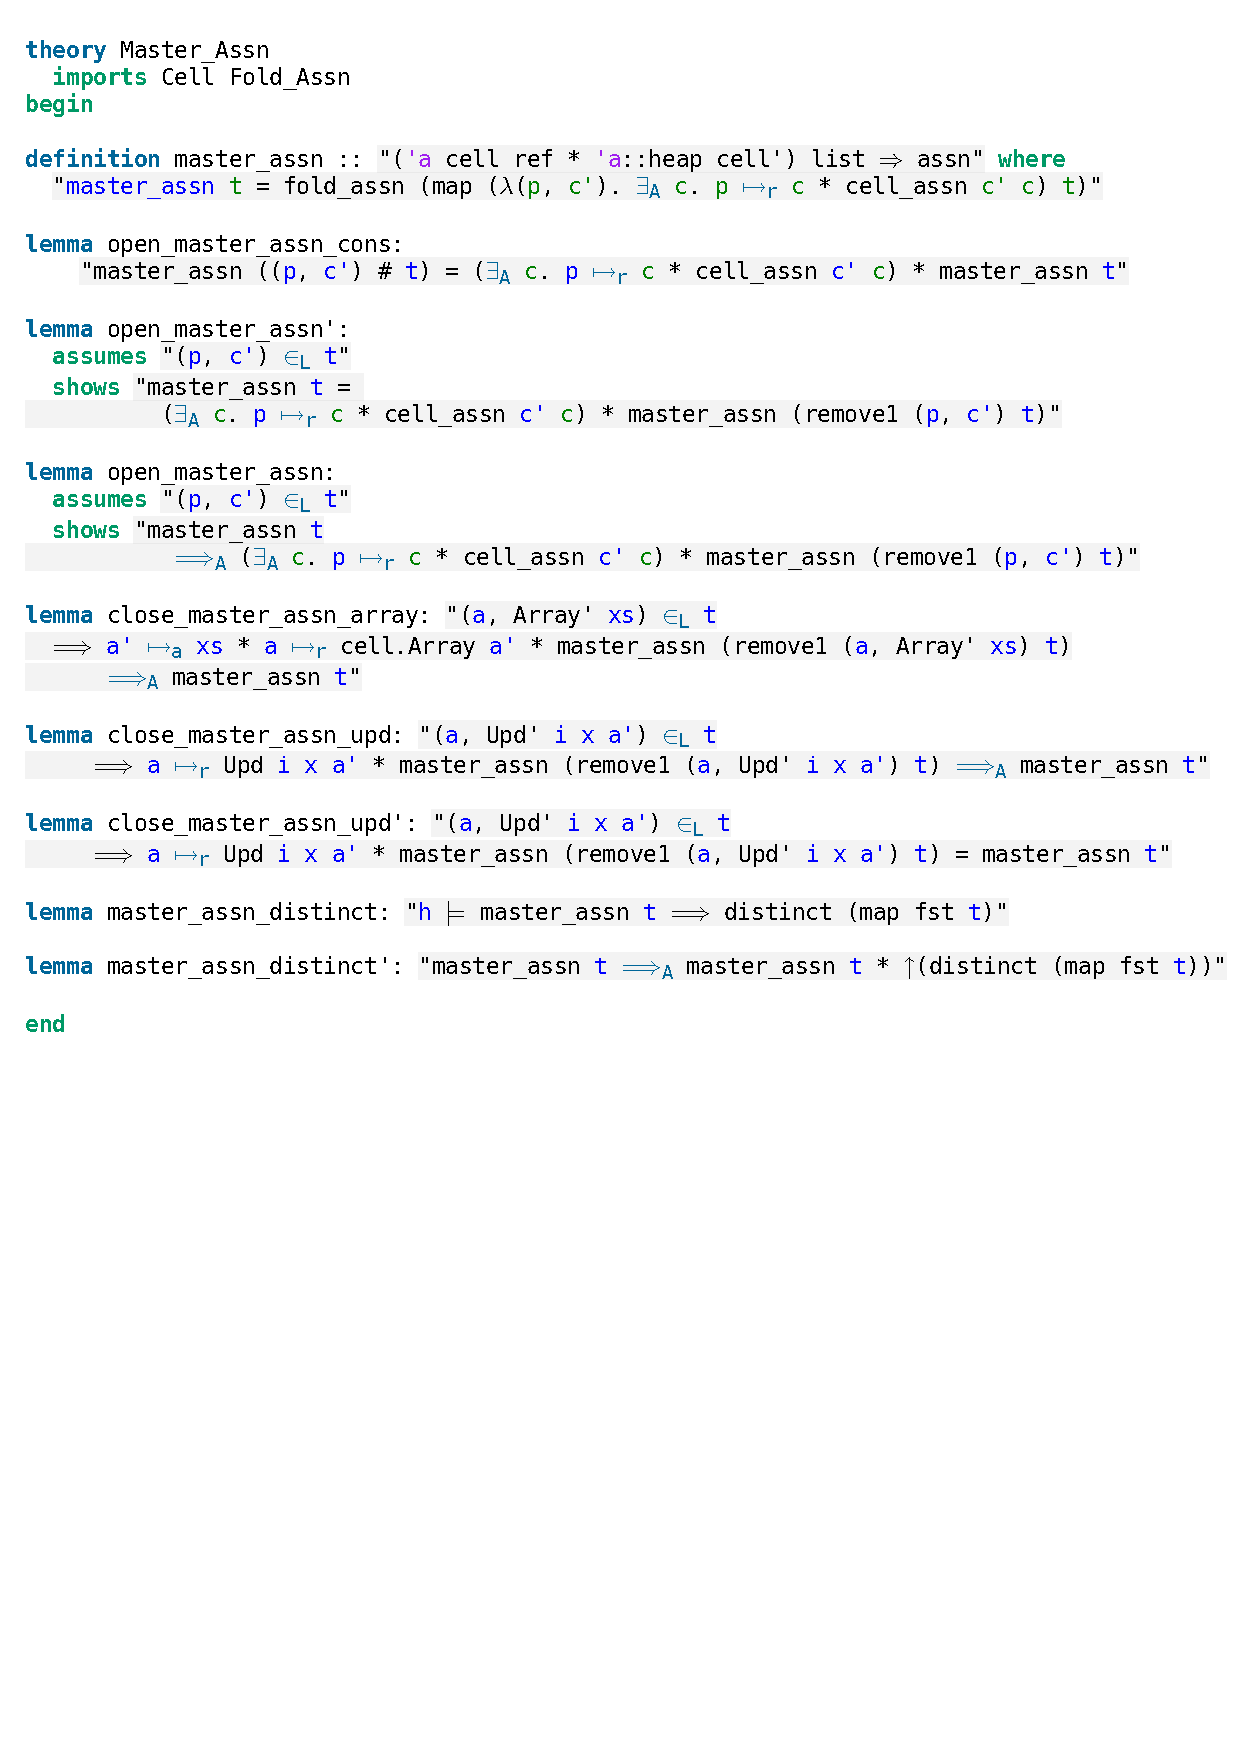
\includegraphics[trim={0 15cm 0 5,4cm}, clip, width=1.00\textwidth]{figures/Theory_Master_Assn.pdf}
    \caption[Master assertion lemmas]{Opening and closing master assertions}
    \label{fig:master_assn_lemmas}
\end{figure}

\noindent We will use these lemmas extensively to verify the diff array operations by opening and closing the master assertion using the diff array relation. \\
Another important property of master assertions is that all |cell| references in |t| must be distinct (\autoref{fig:master_assn_distinct}). If that is not the case, two assertions with the same pointer would be separated, which in separation logic always results in |false|.

\begin{figure}[htpb]
    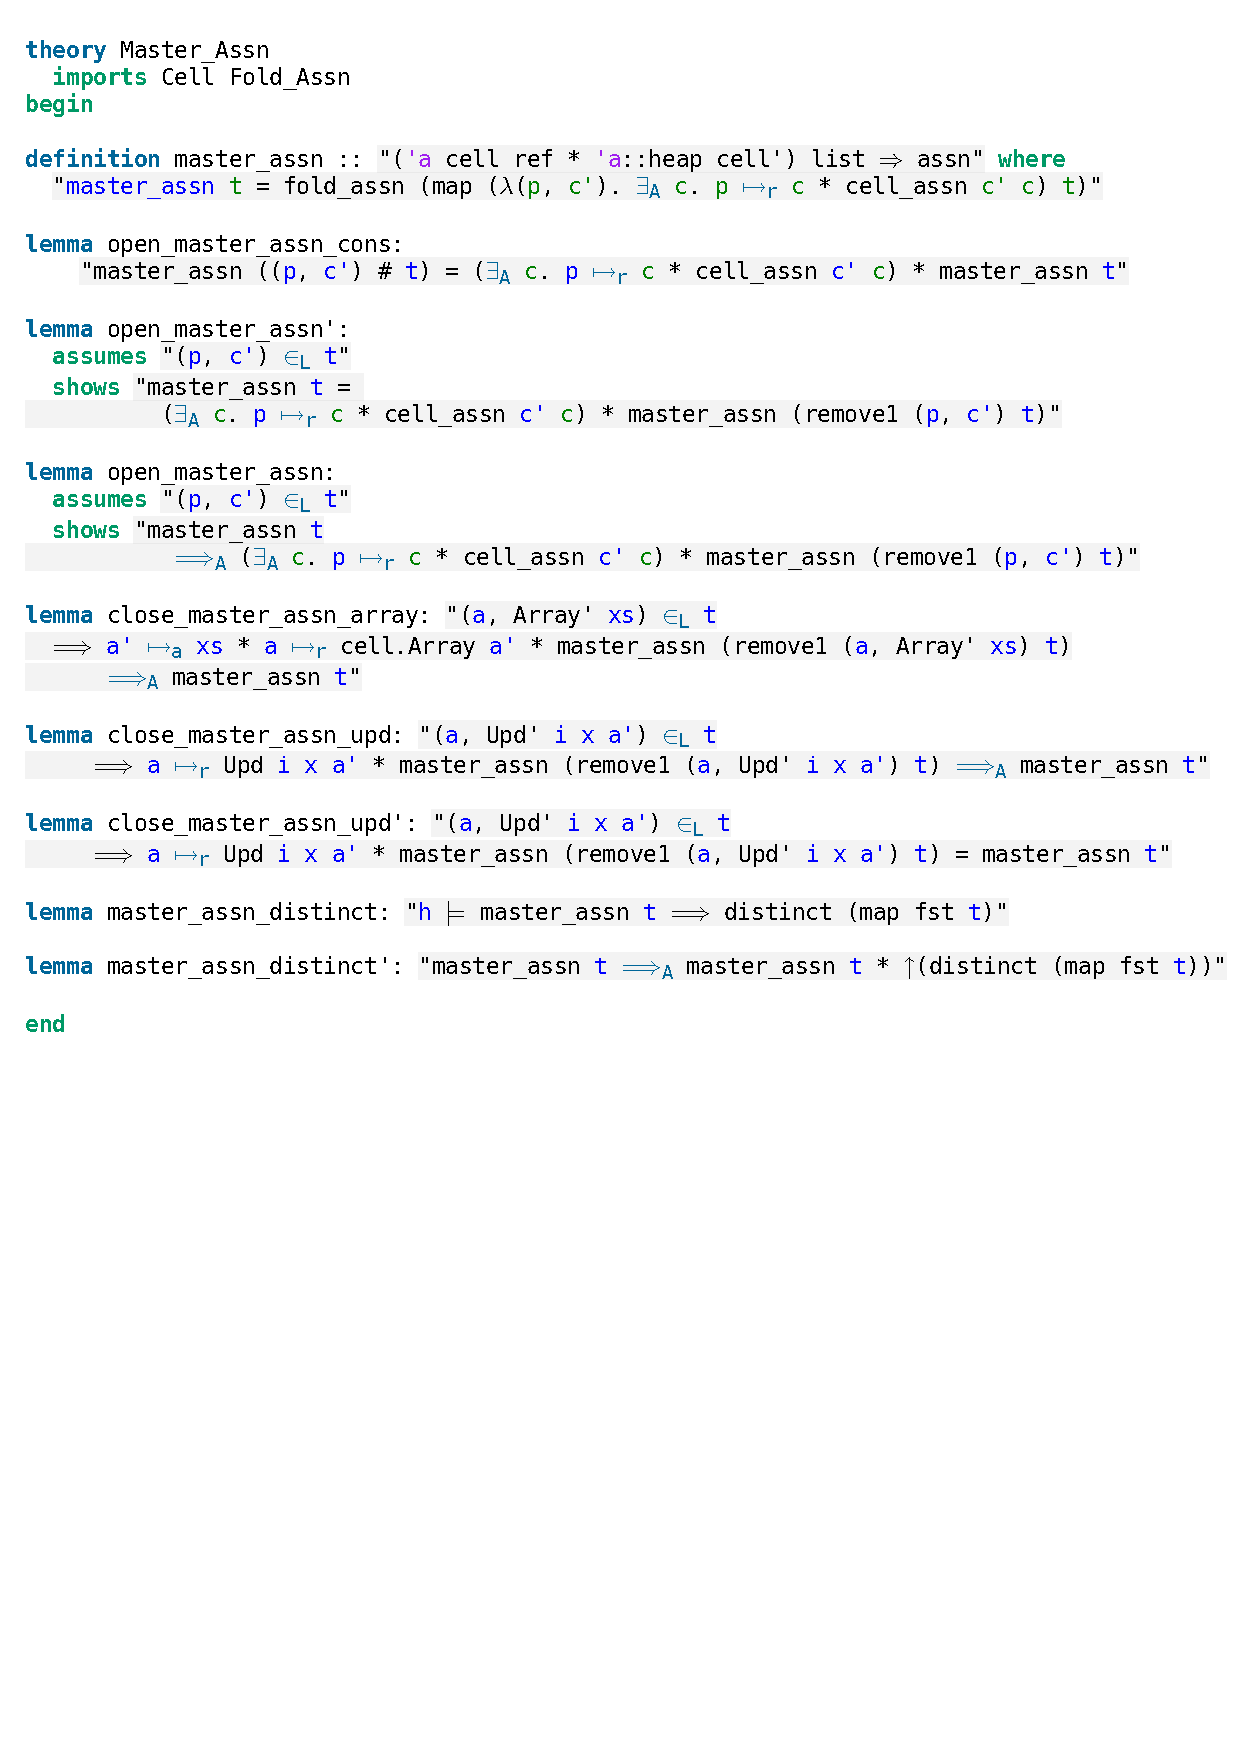
\includegraphics[trim={0 13,1cm 0 15,2cm}, clip, width=1.00\textwidth]{figures/Theory_Master_Assn.pdf}
    \caption[Pointers in a master assertion are distinct]{Pointers in a master assertion are distinct}
    \label{fig:master_assn_distinct}
\end{figure}

\section{Diff Array Operations}\label{section:diff_arr_operations}

In the following, we will use references to cells as diff arrays and create a type synonym for that (\autoref{fig:diff_arr_type_synonym}).

\begin{figure}[htpb]
    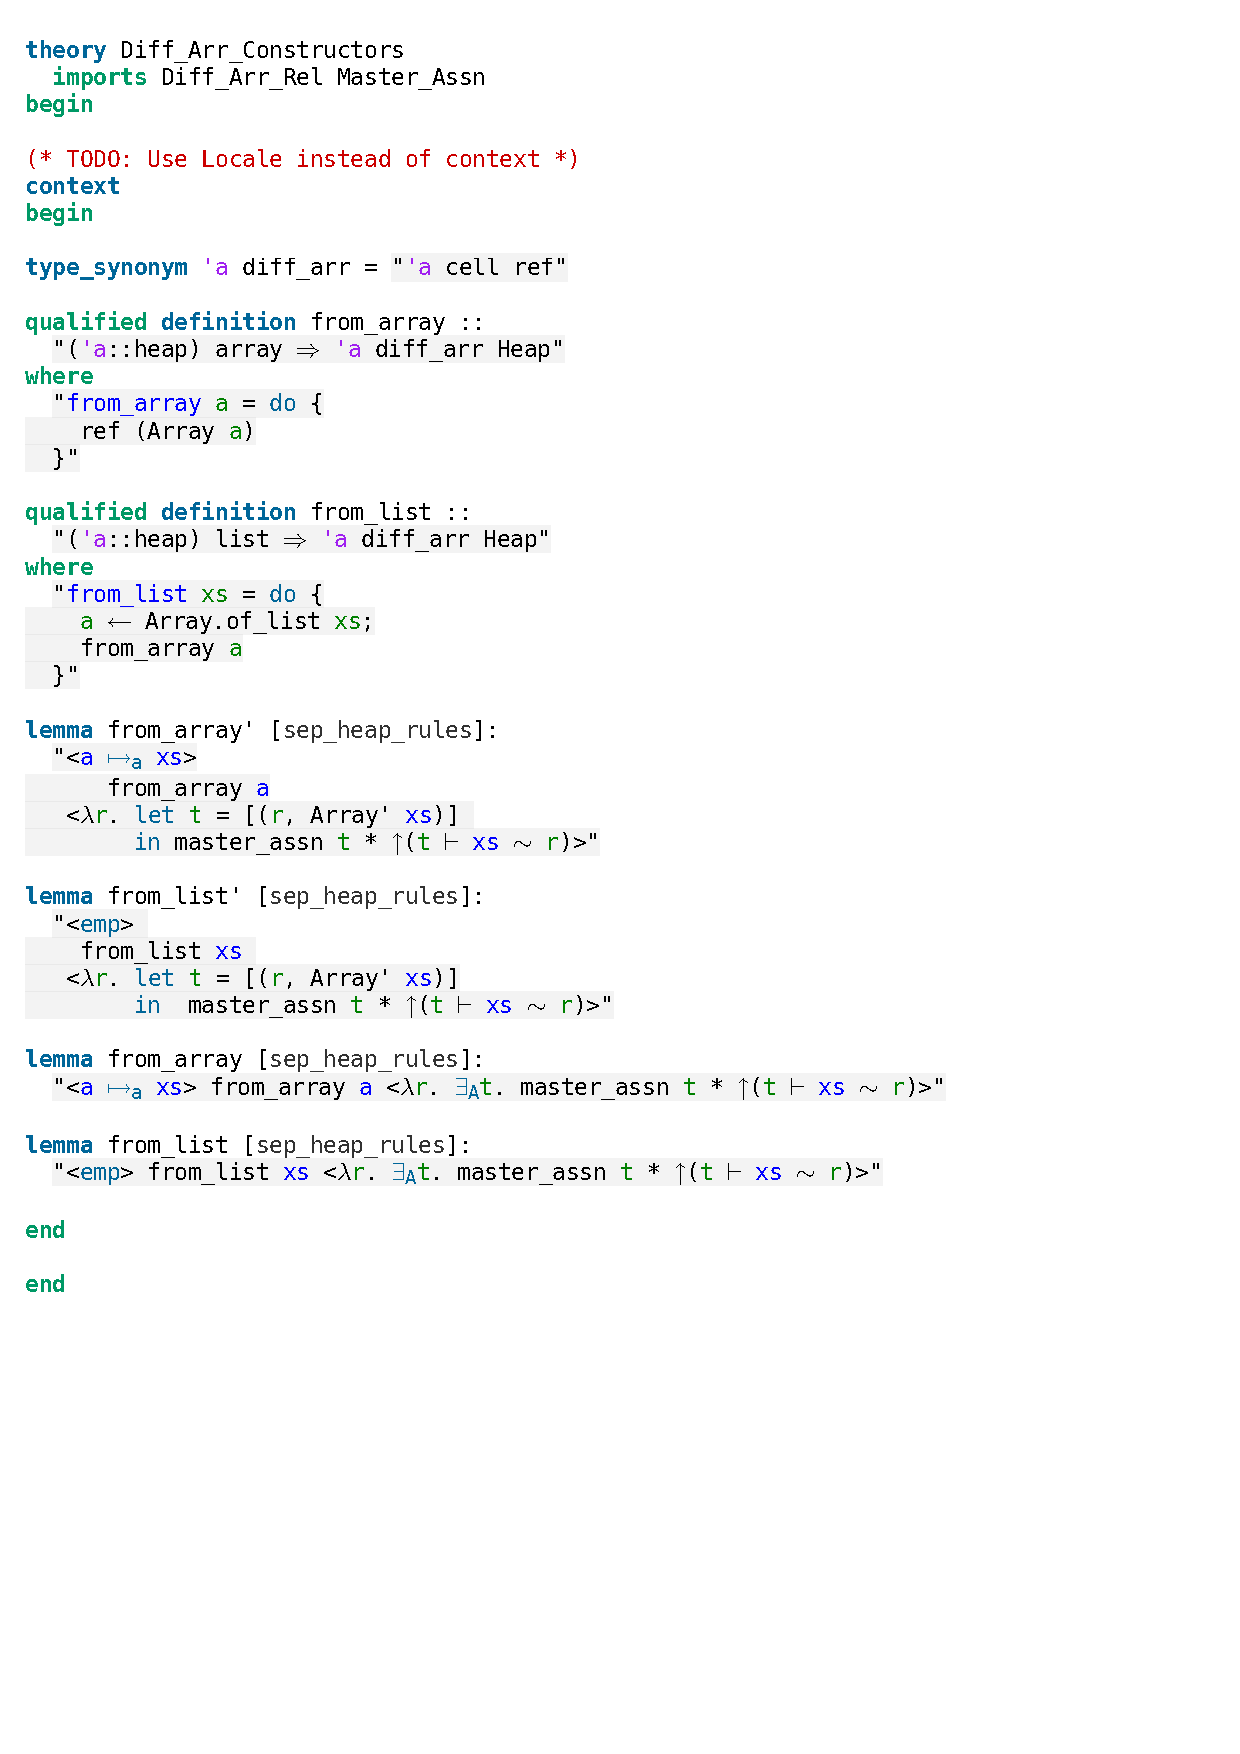
\includegraphics[trim={0 24,9cm 0 4,1cm}, clip, width=1.00\textwidth]{figures/Theory_Diff_Arr_Constructors.pdf}
    \caption[Diff array type synonym]{Diff array type synonym}
    \label{fig:diff_arr_type_synonym}
\end{figure}

\subsection{Constructors}

\begin{figure}[htpb]
    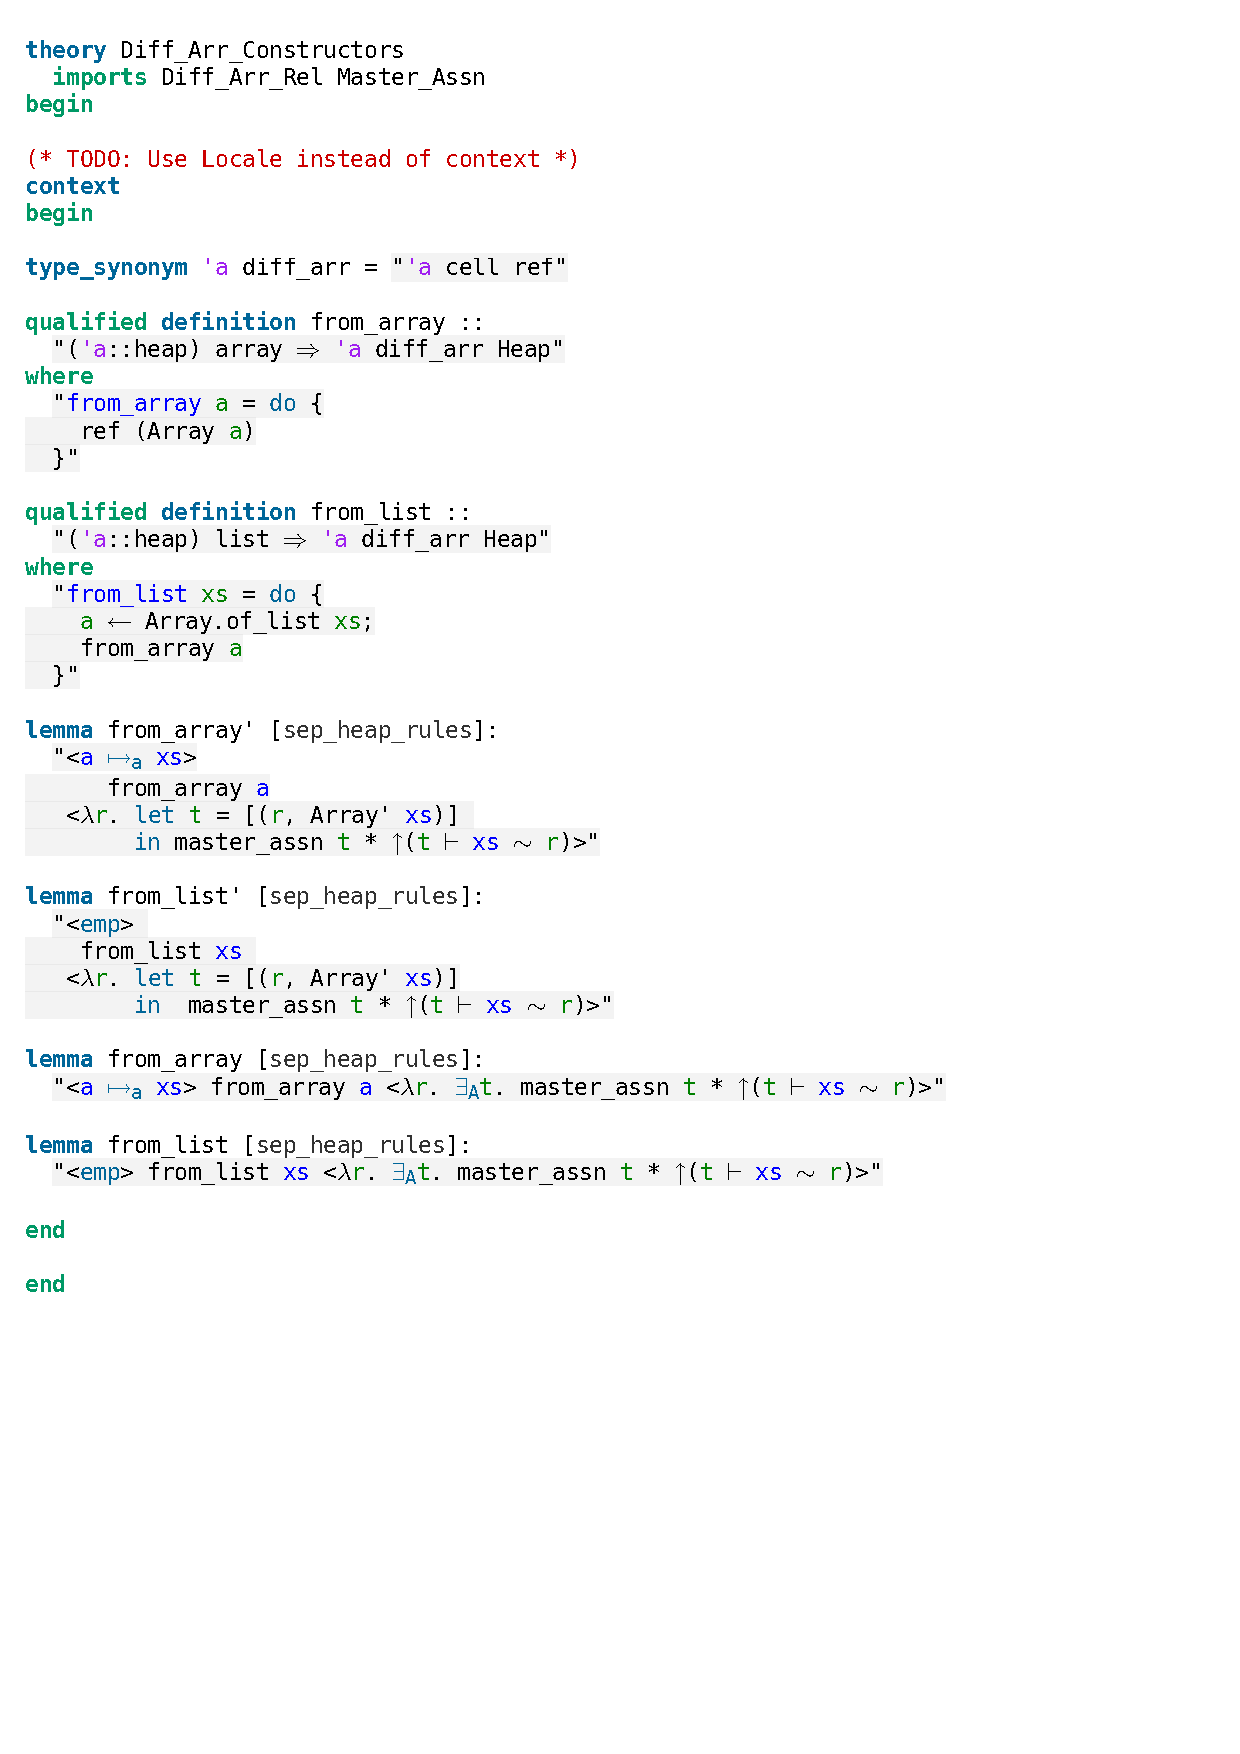
\includegraphics[trim={0 18cm 0 5,2cm}, clip, width=1.00\textwidth]{figures/Theory_Diff_Arr_Constructors.pdf}
    \caption[Diff array constructors]{Diff array constructors}
    \label{fig:diff_arr_constructors}
\end{figure}

\noindent For creating diff arrays from plain arrays and lists, we define two constructor functions (\autoref{fig:diff_arr_constructors}). The latter creates a plain array of the list and then uses the former, which simply creates an |Array|-cell and then returns a reference to it.\\
To verify imperative implementations, we use Hoare triples, as introduced in \autoref{chapter:separation-logic}. When creating a new diff array, a new master assertion, as well as a new diff array relation, are introduced in the postcondition of the Hoare triple. We have two versions of the proofs (\autoref{fig:diff_arr_constructor_proofs}), once with concrete |t|s and once existentially quantified over |t|, because later, we mostly will not care about the concrete |t|s anymore. The preconditions of the list proofs are empty, meaning that the list constructors can be called everywhere. The array proofs have an array pointer assertion as their precondition, which is naturally introduced when arrays are created.

\begin{figure}[htpb]
    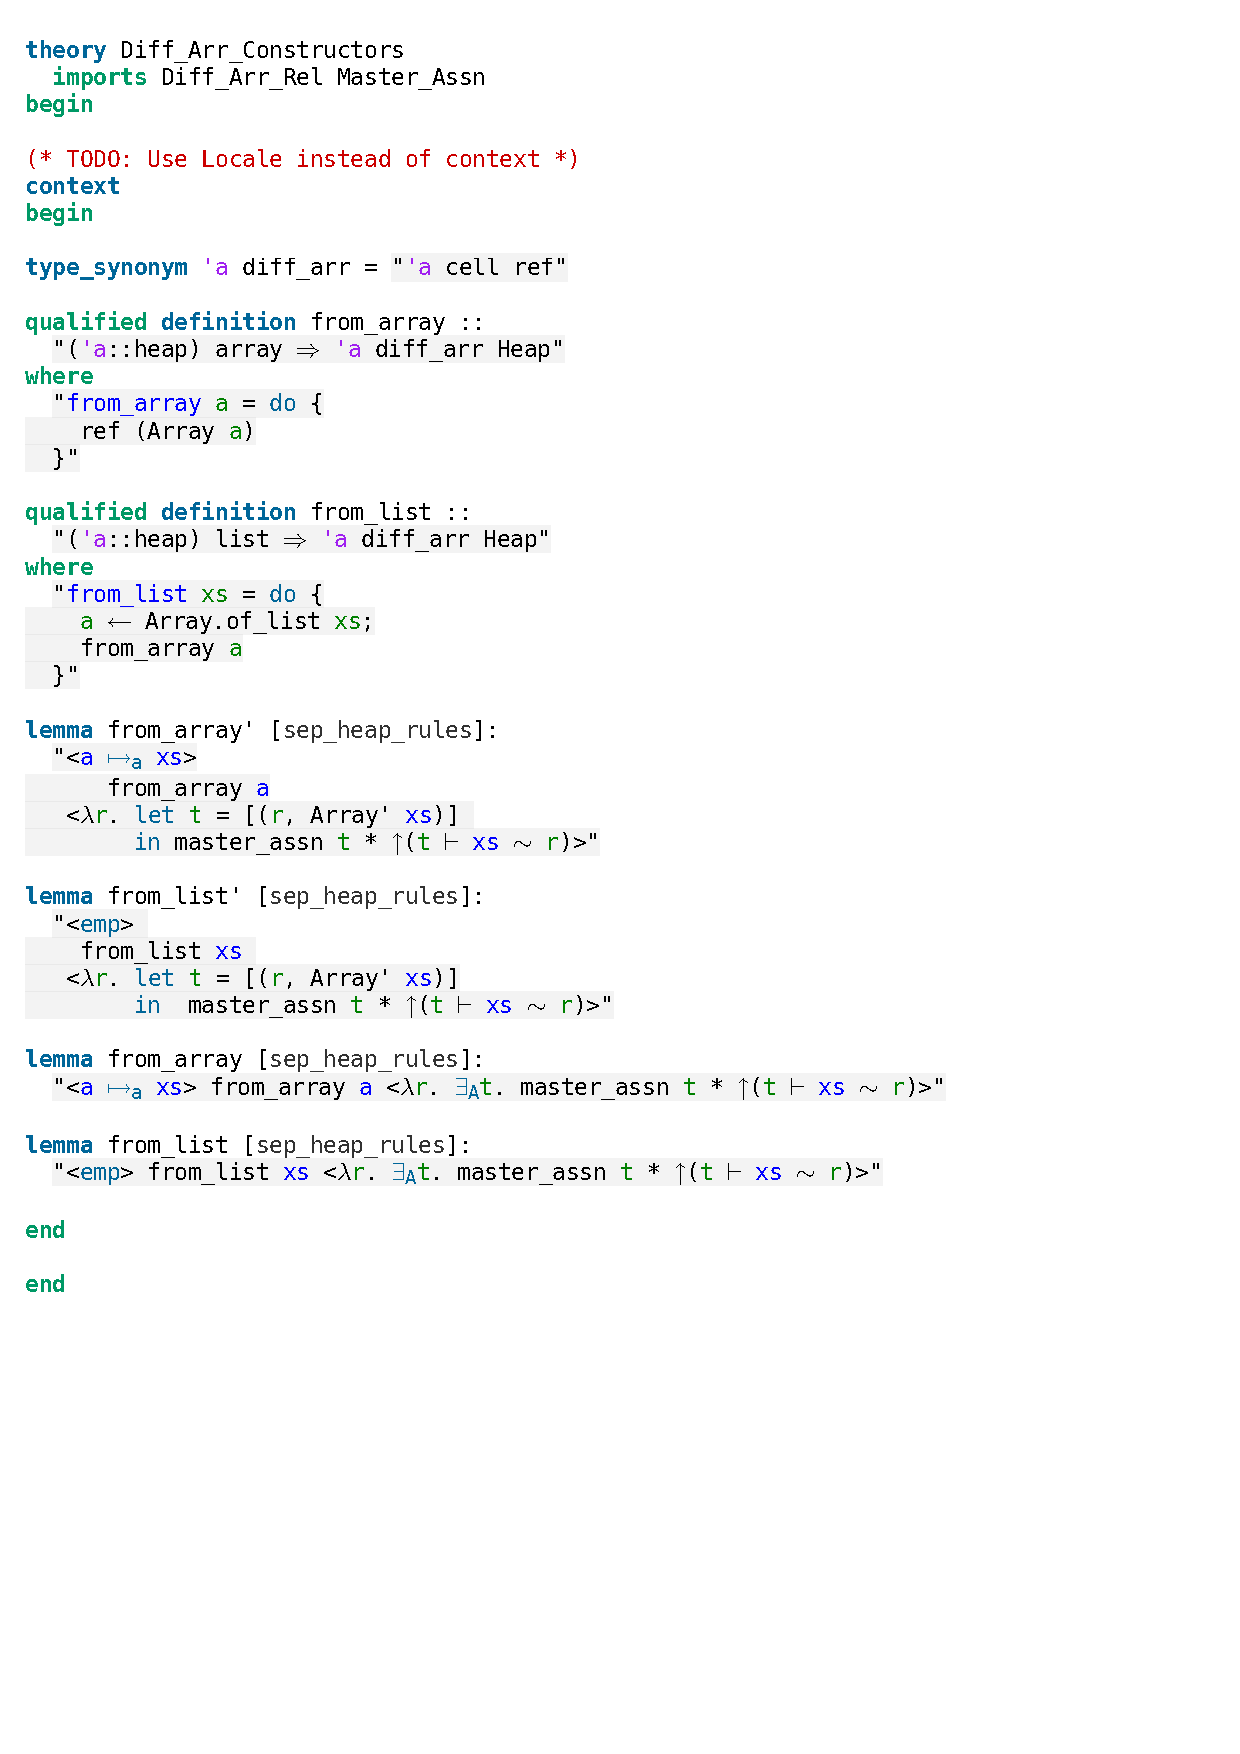
\includegraphics[trim={0 9,6cm 0 12,2cm}, clip, width=1.00\textwidth]{figures/Theory_Diff_Arr_Constructors.pdf}
    \caption[Diff array constructor proofs]{Diff array constructor proofs}
    \label{fig:diff_arr_constructor_proofs}
\end{figure}

\noindent The proofs are all based on |from|\_|array|', which we prove by providing instances for the existential quantifications of the master assertion and the diff array relation. The unfolded master assertion says that the reference returned by the constructor function needs to point to an |Array| cell and that the array inside the cell needs to point to the provided list. The implementation of the constructor function directly fulfils these two requirements. To also fulfill the diff array relation, we instantiate the length of the update list with zero since we have no updates yet. In its base case, the diff array relation requires the cell and its list abstraction to be in |t|, which is true because |t| is the singleton list containing precisely this pair of values.

\subsection{Lookup}

After constructing a diff array, we also want to be able to look up values in it (\autoref{fig:diff_arr_lookup}). For that, we first check if we are at a leaf node. If yes, we look the value up in the underlying array. Otherwise, we compare the index of the update we are looking at with the index of the value we want to look up. In case they equal, we can directly return the value of the update, or else we recurse on the diff array to which the update is pointing.

\begin{figure}[htpb]
    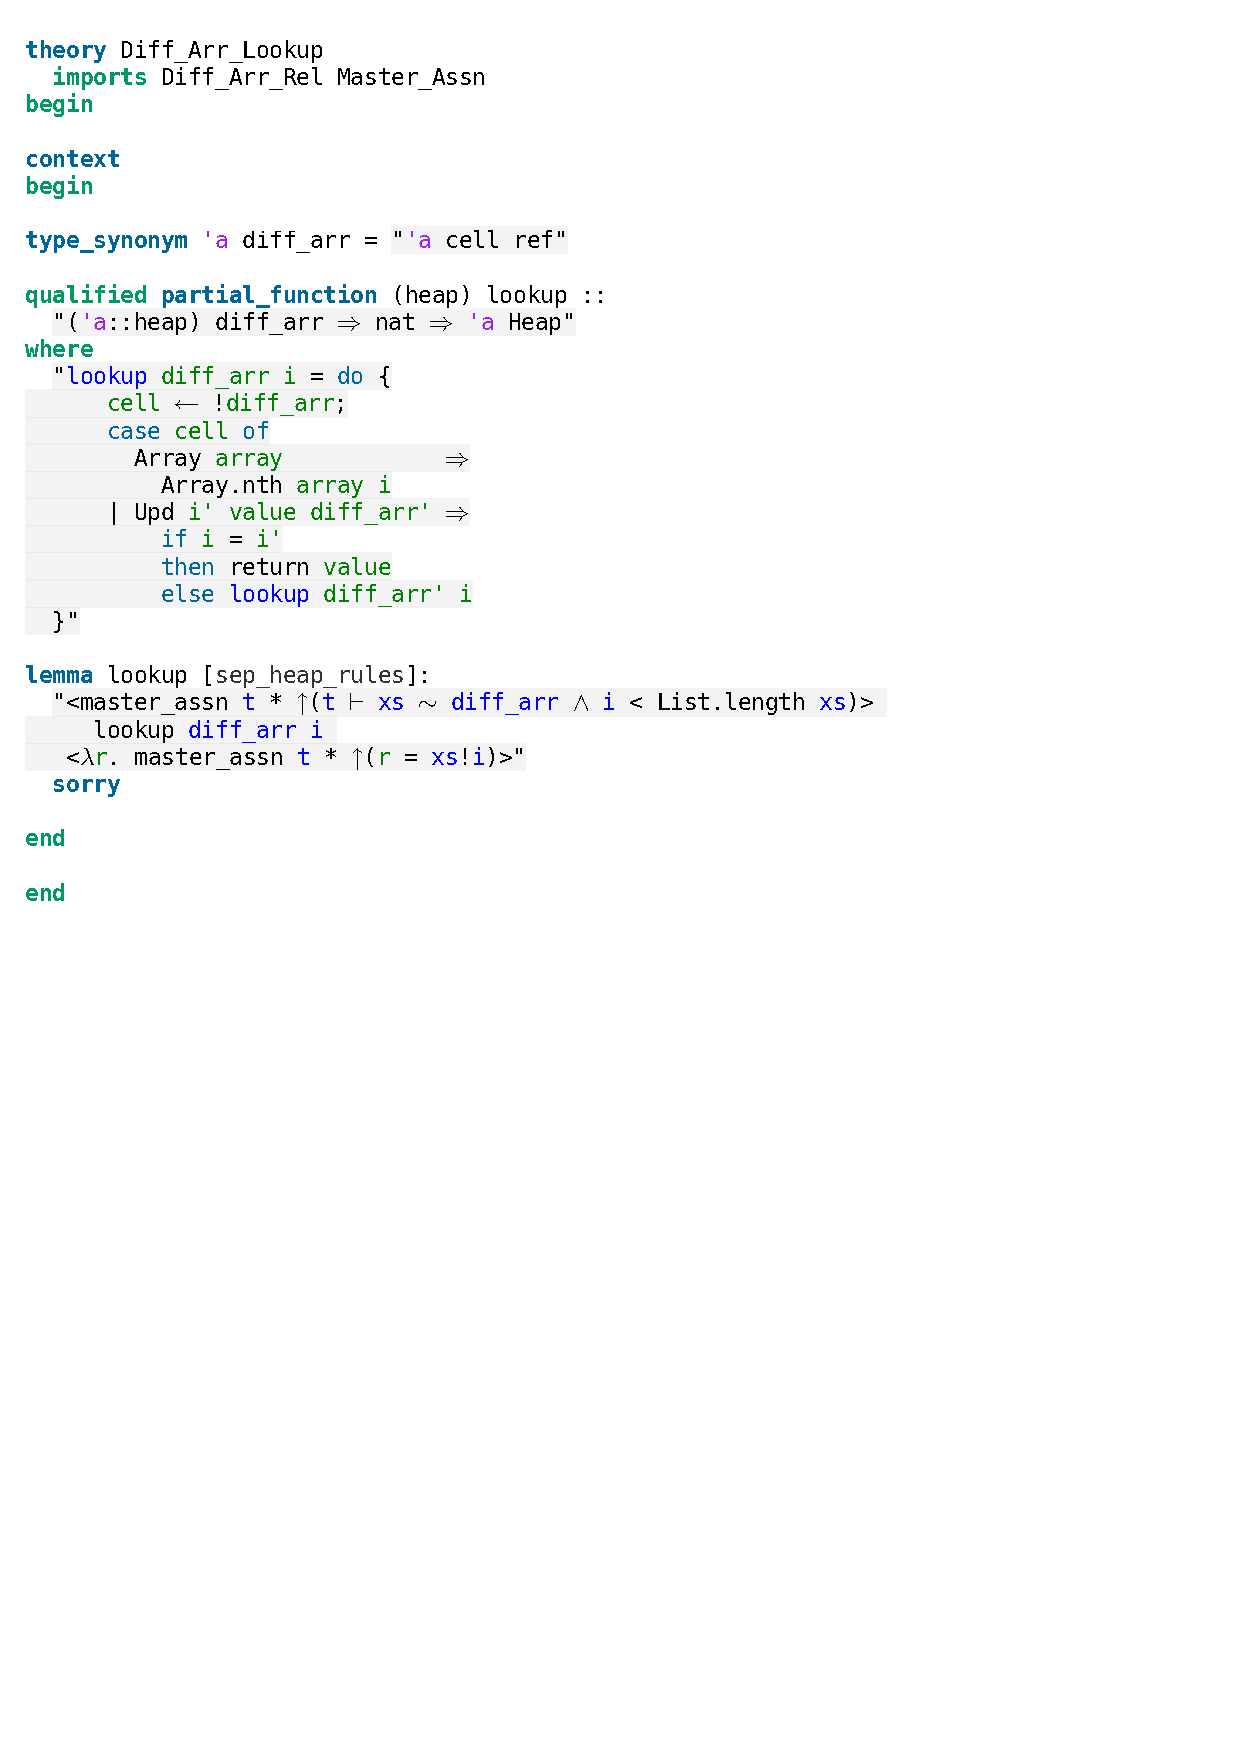
\includegraphics[trim={0 19cm 0 4,8cm}, clip, width=1.00\textwidth]{figures/Theory_Diff_Arr_Lookup.pdf}
    \caption[Diff array lookup]{Diff array lookup}
    \label{fig:diff_arr_lookup}
\end{figure}

\noindent To prove the implementation correct (\autoref{fig:diff_arr_lookup_proof}), we assume a master assertion, a diff array, and that the index we want to look up is in the array's bounds. After a function execution, the same master assertion should hold, and the result of the function should yield the same value as the list abstraction at that index.

\begin{figure}[htpb]
    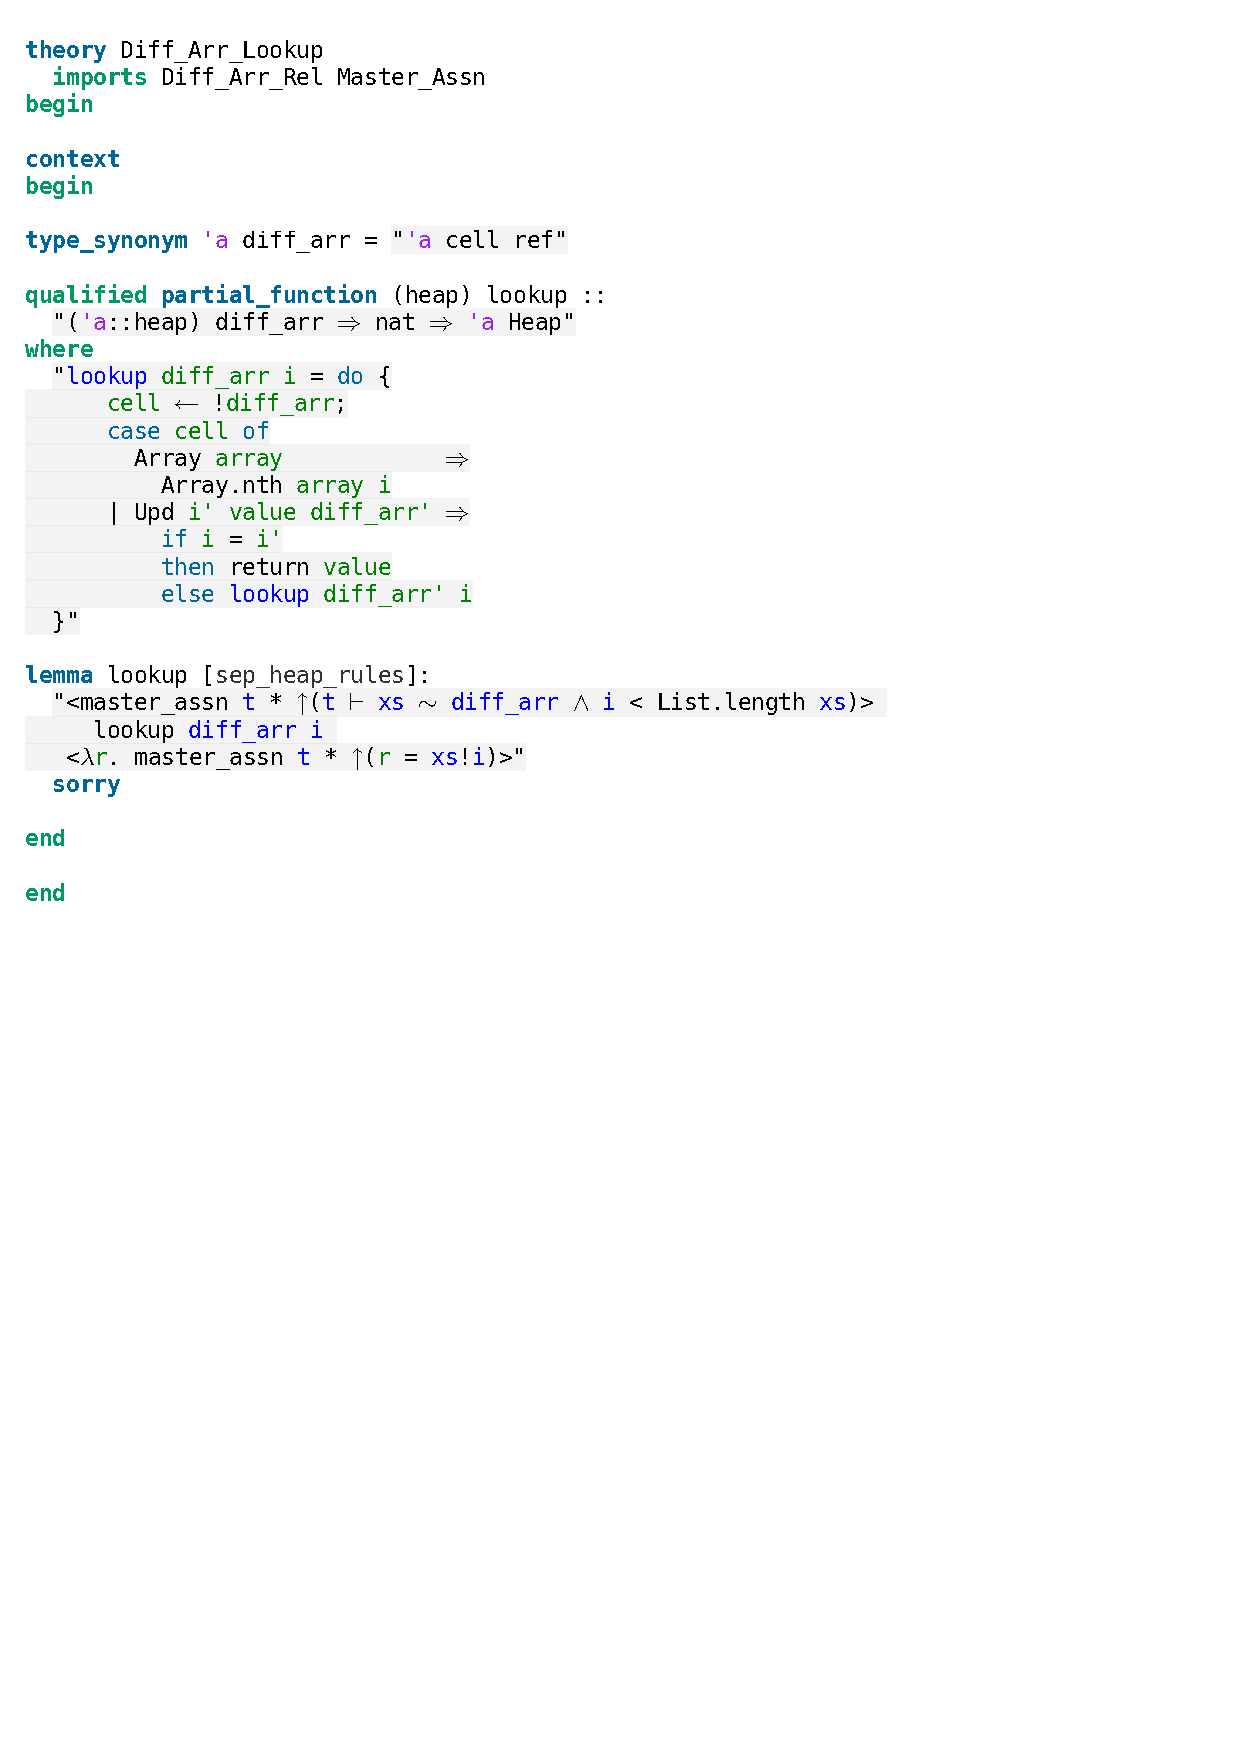
\includegraphics[trim={0 16,6cm 0 11,2cm}, clip, width=1.00\textwidth]{figures/Theory_Diff_Arr_Lookup.pdf}
    \caption[Diff array lookup proof]{Diff array lookup proof}
    \label{fig:diff_arr_lookup_proof}
\end{figure}

\noindent The proof is an induction on the number of updates of the diff array. After opening the master assertion for the current diff array cell, the separation logic automation can prove both cases of the induction.

\subsection{Update}

For updating diff arrays (\autoref{fig:diff_arr_update}), we follow the heuristic of \cite[p.27]{Bloss1989}, that the most recent version of an array is mainly accessed. Consequentially, when updating an array without an update tree, we update destructively and create a new pointer as the most recent version. The previous version gets updated by assigning it an update cell containing the reverted update and a pointer to the new version. Following the same schema, we realize arrays, which have an update tree and then update the newly created arrays destructively.

\begin{figure}[htpb]
    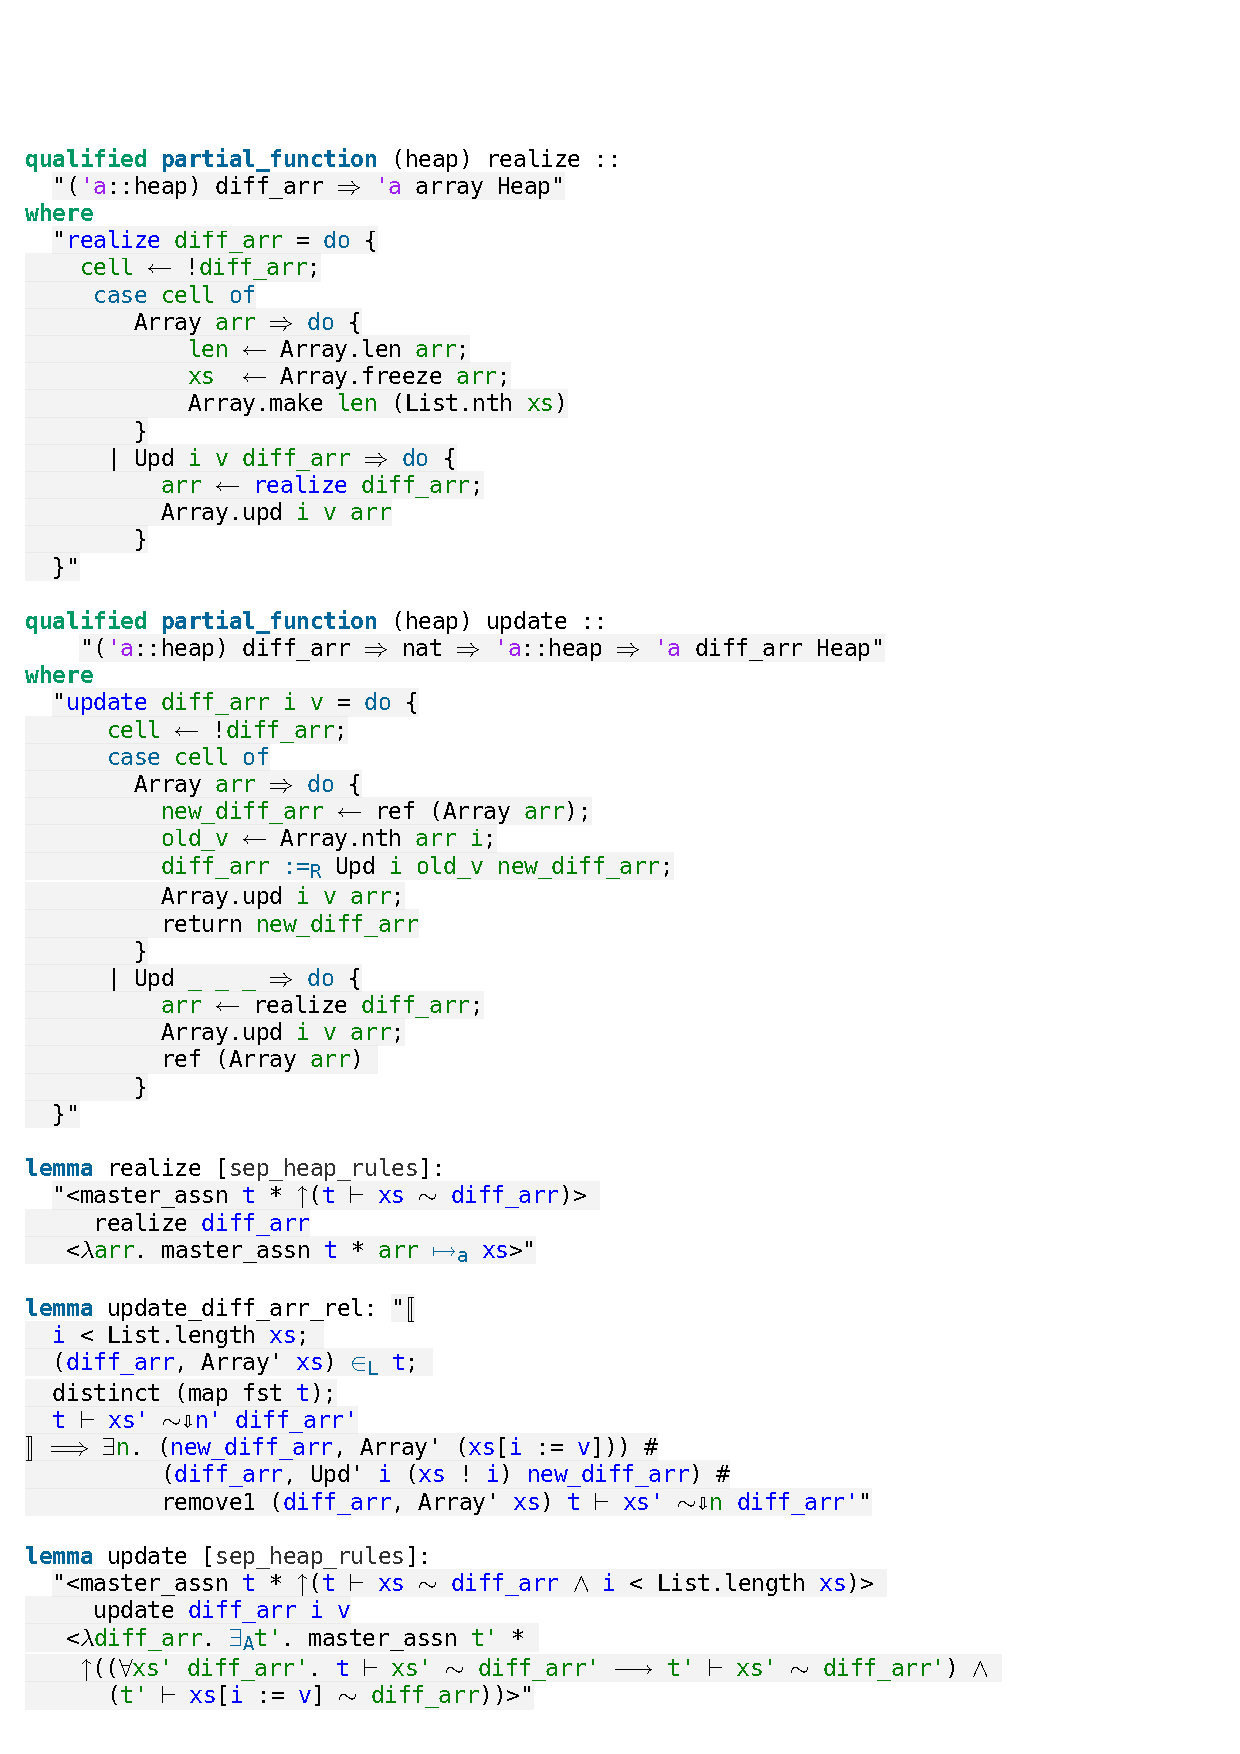
\includegraphics[trim={0 10,6cm 0 10,2cm}, clip, width=1.00\textwidth]{figures/Theory_Diff_Arr_Update.pdf}
    \caption[Diff array update]{Diff array update}
    \label{fig:diff_arr_update}
\end{figure}

\noindent By realizing, we mean creating a new array with the updates of the update tree applied. Like this, we can guarantee that accesses to the most recent versions always have a runtime of $\mathcal{O}(1)$. \\
The utilized |realize| function (\autoref{fig:diff_arr_realize}) recurses the update tree down to the plain array, copies it, and applies the updates of the update tree destructively to the copy.

\begin{figure}[htpb]
    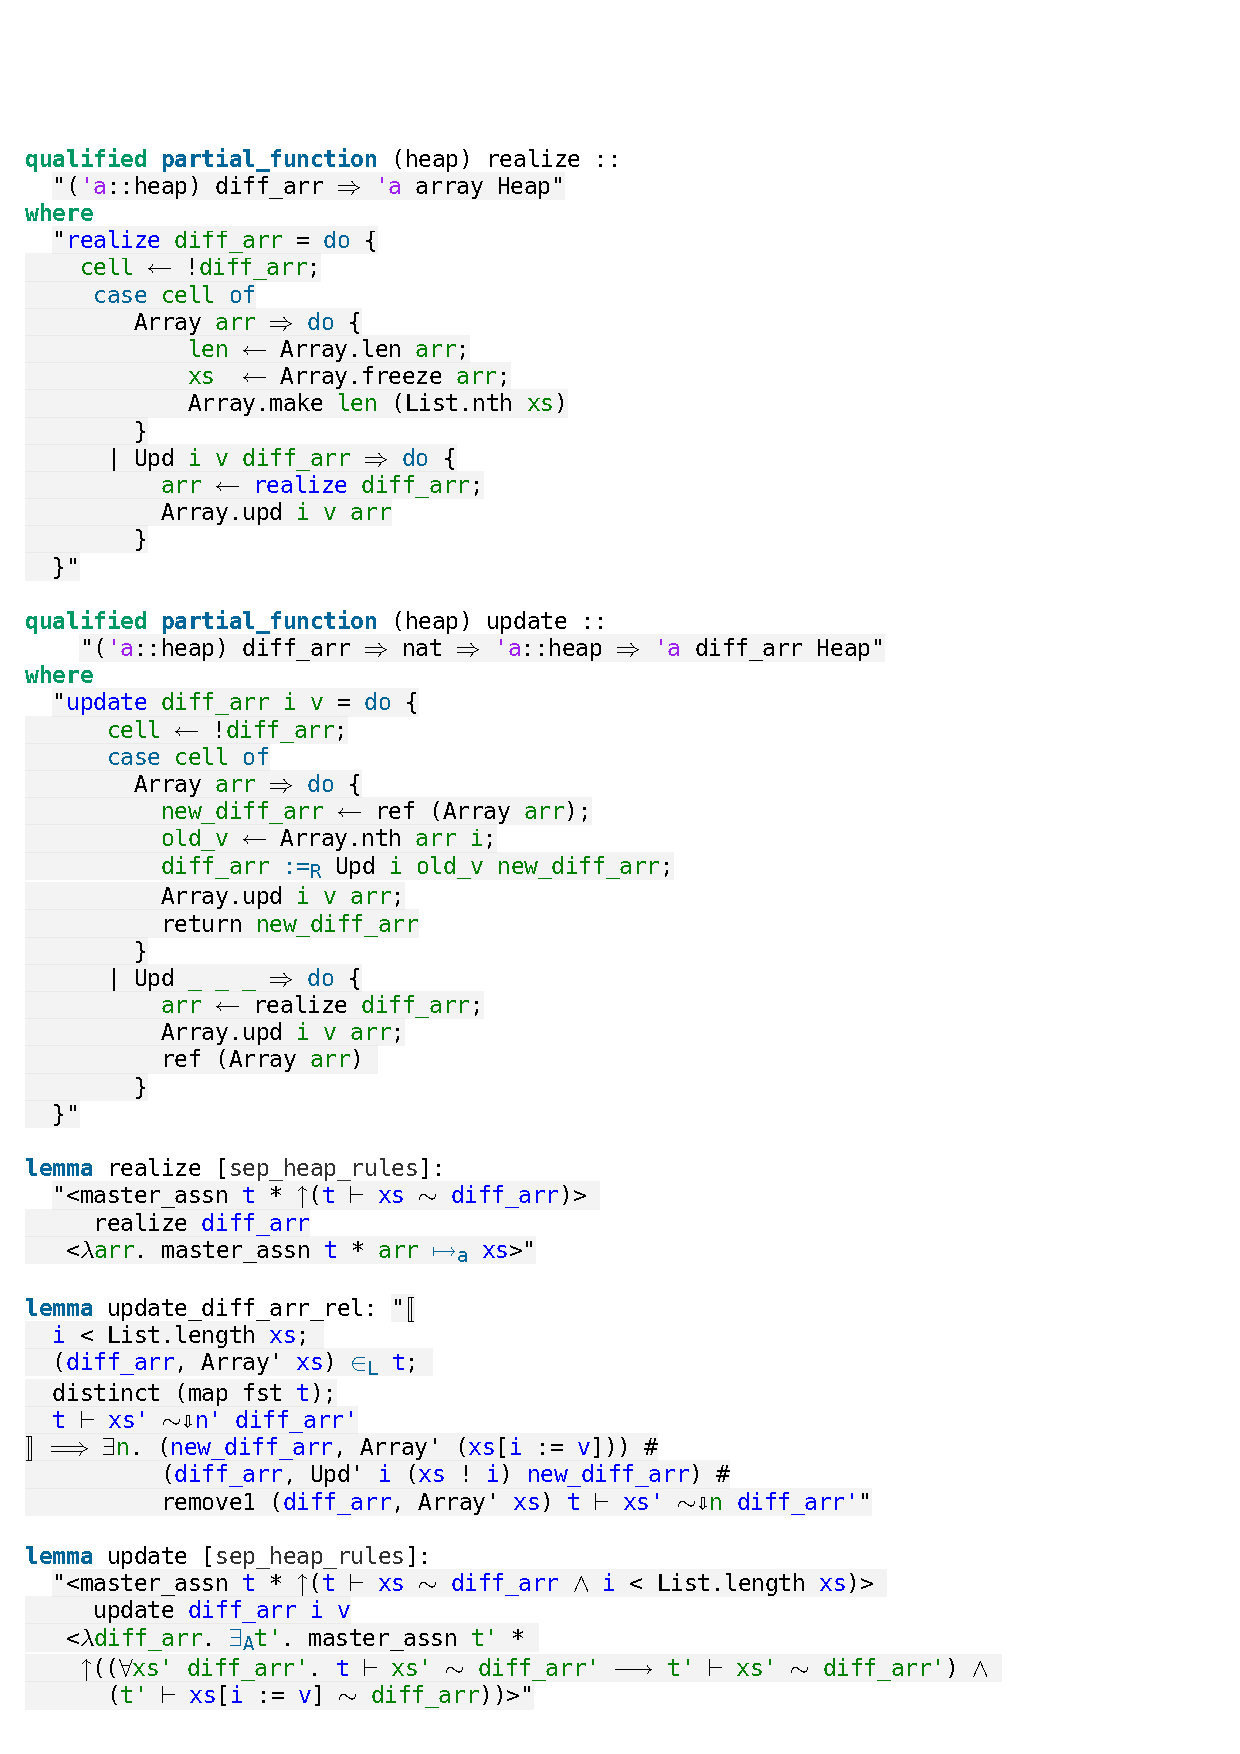
\includegraphics[trim={0 19,8cm 0 2,4cm}, clip, width=1.00\textwidth]{figures/Theory_Diff_Arr_Update.pdf}
    \caption[Realize diff array]{Realize diff array}
    \label{fig:diff_arr_realize}
\end{figure}

\noindent We prove |realize| again by induction on the number of updates of the diff array (\autoref{fig:diff_arr_realize_proof}). To resolve the case distinction on the |cell| type, we can, in the base case as well as the induction step, open the master assertion. After knowing what kind of cell we are looking at currently, we can close the master assertion again and the separation logic automation can prove that the function preserves the master assertion and additionally creates a plain array that contains the same elements as the diff array.

\begin{figure}[htpb]
    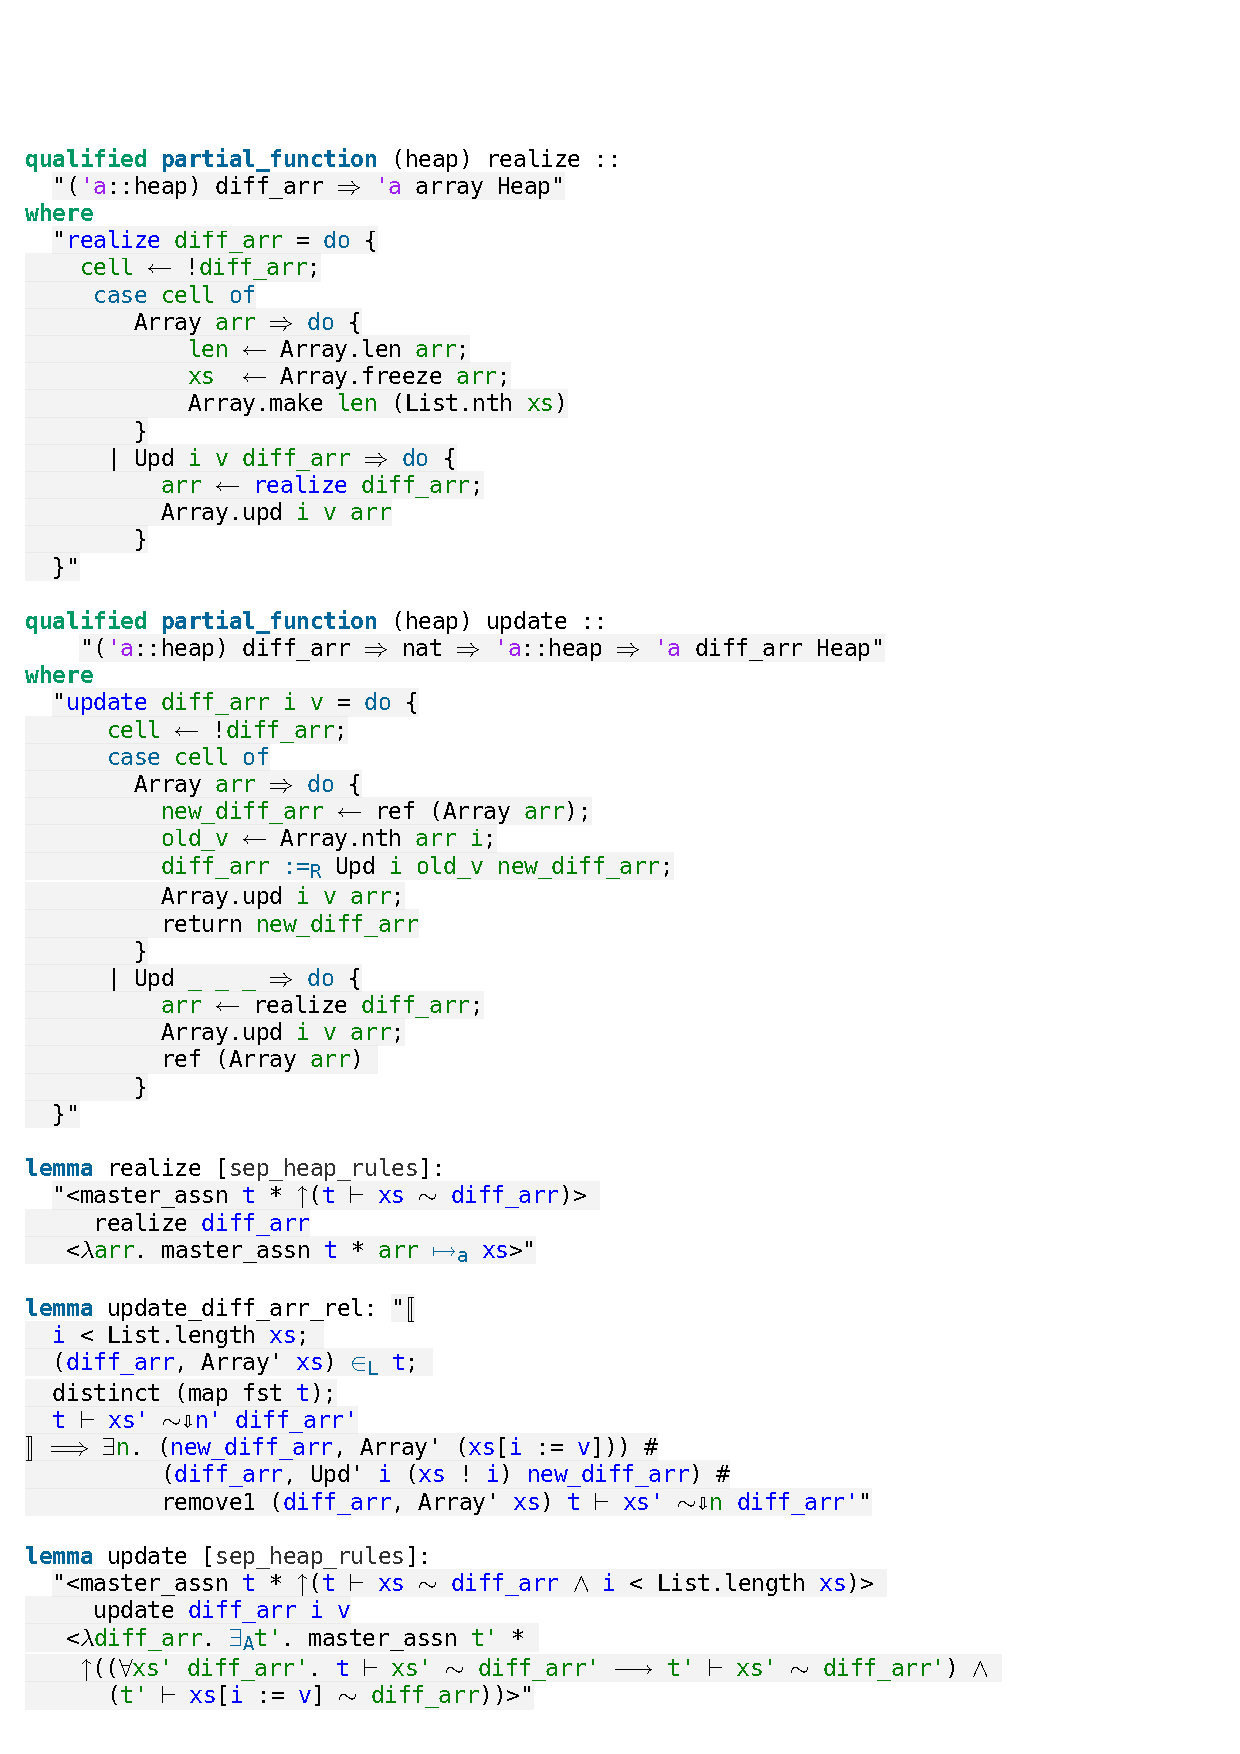
\includegraphics[trim={0 8,2cm 0 19,6cm}, clip, width=1.00\textwidth]{figures/Theory_Diff_Arr_Update.pdf}
    \caption[Diff array realize proof]{Diff array realize proof}
    \label{fig:diff_arr_realize_proof}
\end{figure}

\noindent In order to prove the update operation correct, we first prove an auxiliary lemma (\autoref{fig:diff_arr_rel_update}). It states that a diff array relation still holds if we replace a leaf node with another one that differs in one entry and an update that reverts this difference.

\begin{figure}[htpb]
    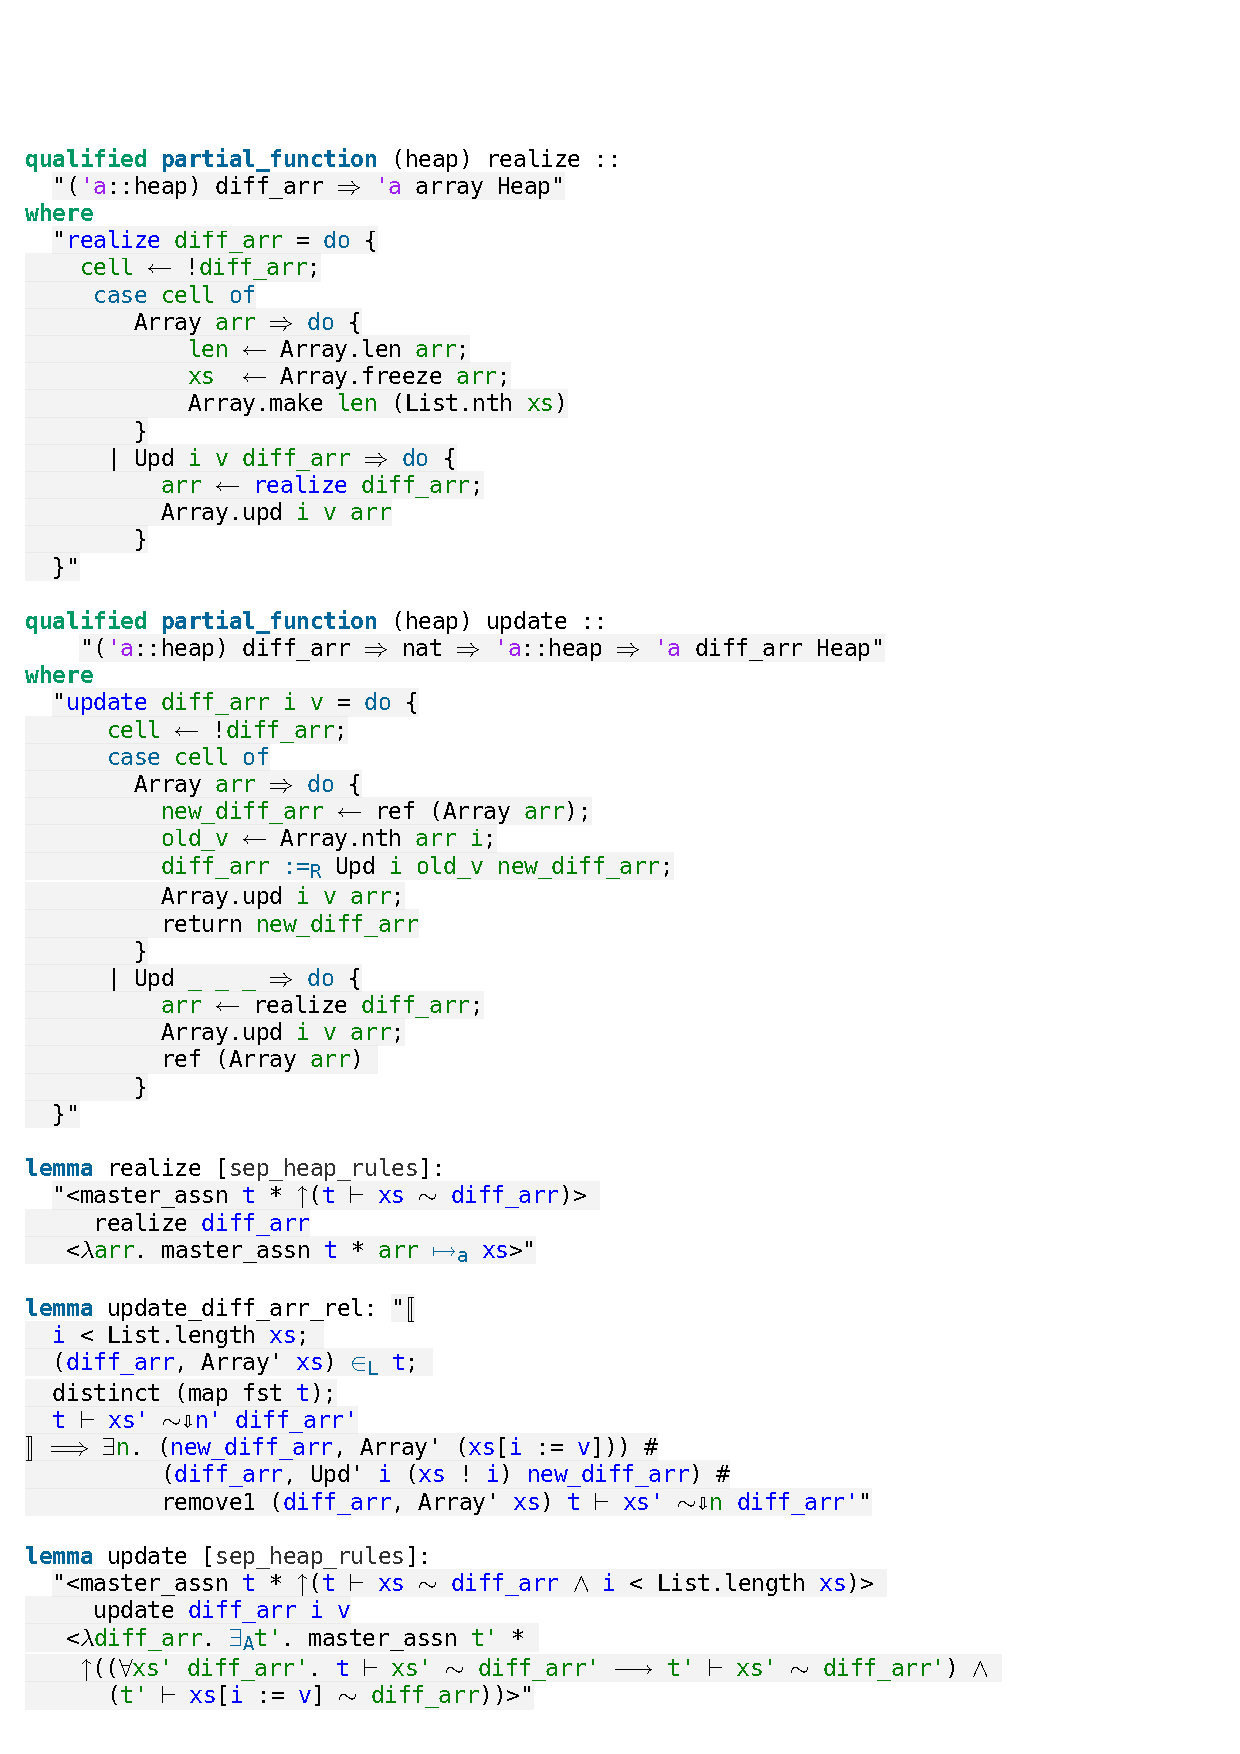
\includegraphics[trim={0 4cm 0 21,8cm}, clip, width=1.00\textwidth]{figures/Theory_Diff_Arr_Update.pdf}
    \caption[Update diff array relation]{Update diff array relation}
    \label{fig:diff_arr_rel_update}
\end{figure}

\noindent An additional assumption is that the |t| under which the diff array relations hold only contains distinct cells. In \autoref{section:master_assn}, we have already shown that a master assertion yields this property.\\
We can prove the lemma using a structural induction on the diff array relation. In the base case, the number of updates that the diff array contains is zero. We can now differentiate two cases: The replaced diff array is the same as the one for which the diff array relation holds or not. We know that the number of updates of the diff array in the diff array relation increases in the first case to one and stays zero in the second. We provide these as the witnesses of the existentially quantified number of updates for the conclusion. The proof automation will then prove the rest.\\
In the induction step of the structural induction, we can unfold one step of the diff array relation. Using the induction hypothesis, we can now show the proposition for the underlying updated array with a fixed number of updates. Finally, we can show the overall conclusion by witnessing the number of updates with the just fixed number incremented by one and using the definition of the diff array relation. This lemma is one of the main building blocks for proving the update operation correct.

\begin{figure}[htpb]
    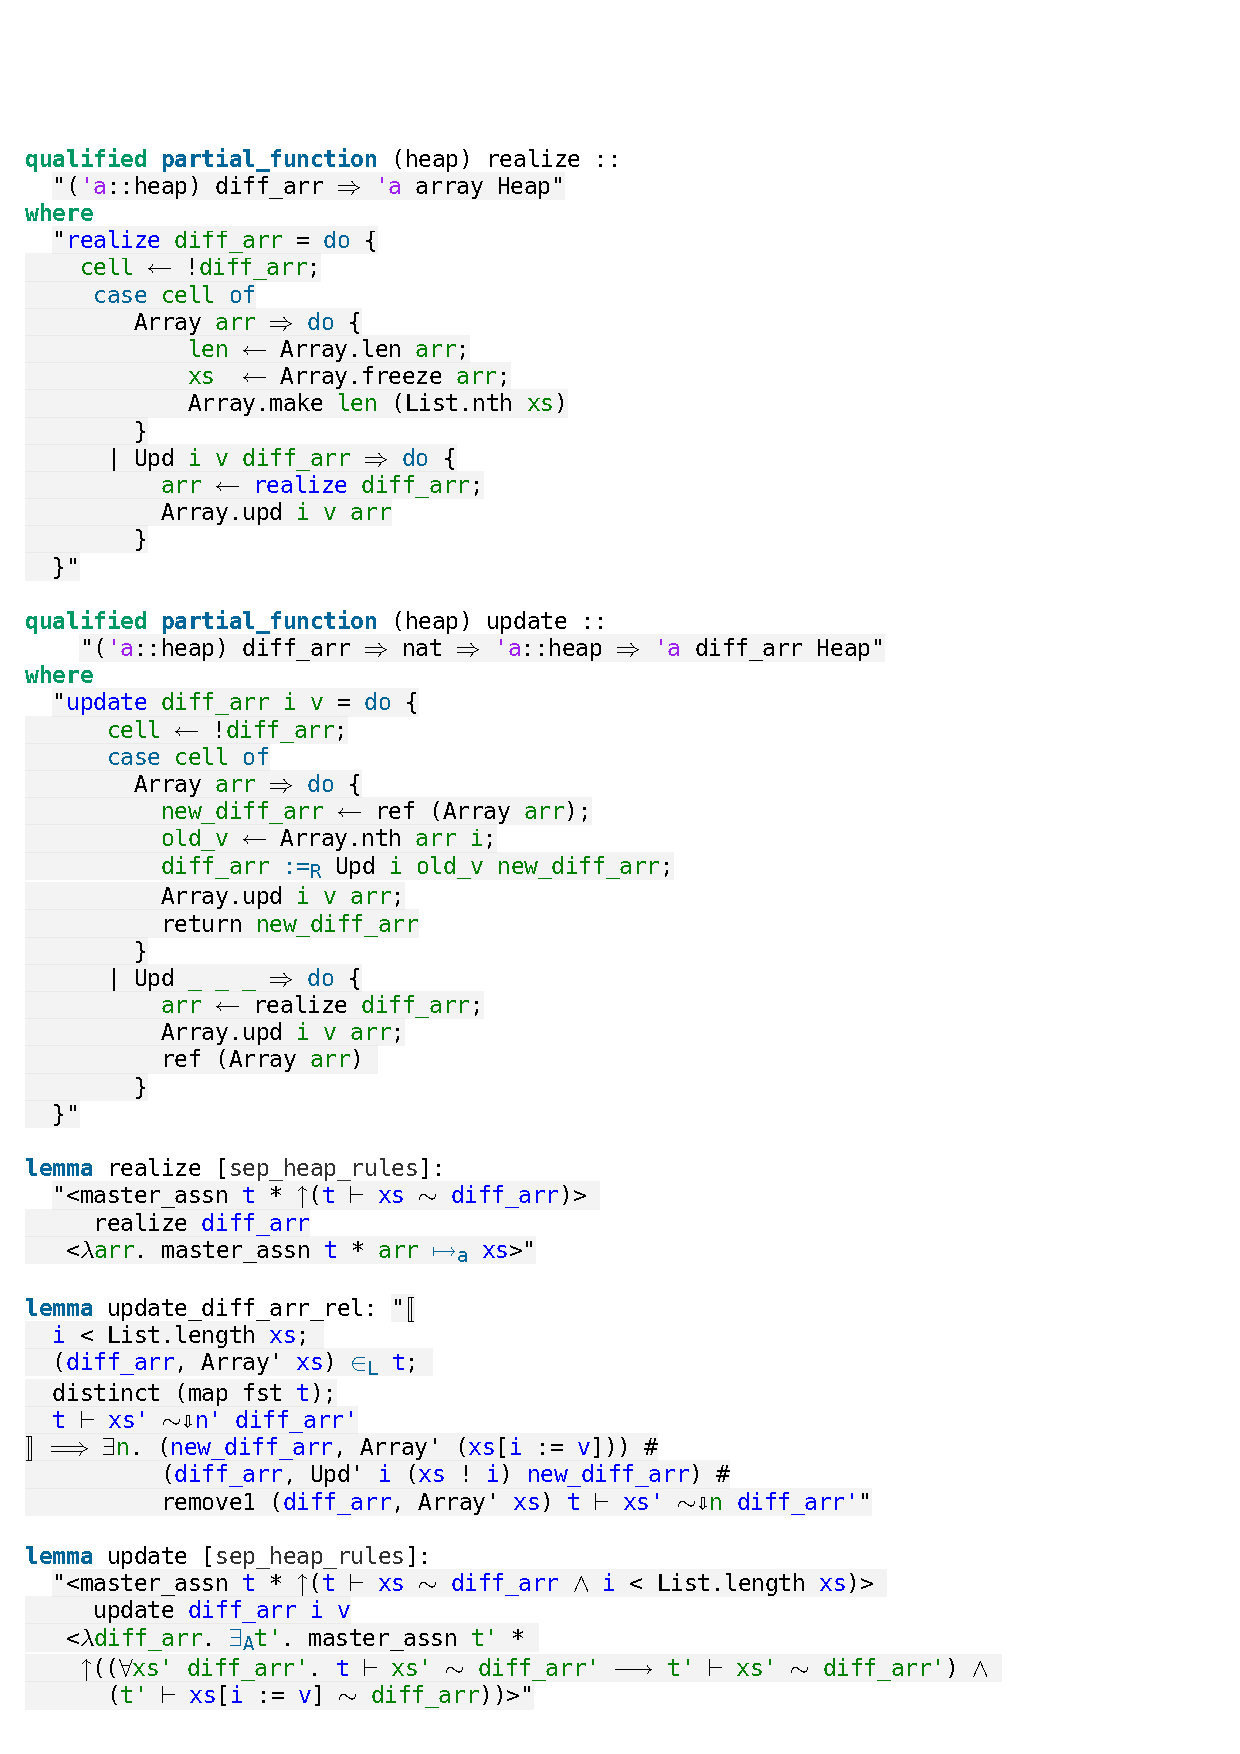
\includegraphics[trim={0 0,7cm 0 26,2cm}, clip, width=1.00\textwidth]{figures/Theory_Diff_Arr_Update.pdf}
    \caption[Diff array update proof]{Diff array update proof}
    \label{fig:diff_arr_update_proof}
\end{figure}

\noindent The lemma of the update operation has the same preconditions as the lookup operation, but its postconditions are slightly more complicated (\autoref{fig:diff_arr_update_proof}). Firstly, there is a new |t|' because the cells of the diff array are not staying the same. The master assertion still needs to hold for it, but the diff array relation now relates the diff array with the updated list. Finally, it is also essential that all the diff array relations that were holding for the |t| of the precondition also hold for the new |t|'. Otherwise, we would lose the old versions of the diff array.\\
To prove this lemma, we differentiate whether the diff array's number of updates is zero. That corresponds to the case distinction on the cell in the function implementation.\\
The easier case\footnote{Because we have already proofs for \lstinline!realize! (\autoref{fig:diff_arr_realize_proof}).} is when the number of updates is not zero, and consequently, the cell is an update cell. Here, we realize the diff array to a new array and then update it. Correspondingly, the proof uses our previous proof for |realize| (\autoref{fig:diff_arr_realize_proof}) and the Imperative/HOL-library proof for destructive array updates. We now know that the master assertion still holds for |t| and, additionally, that there is a new diff array that relates to the list updated at index |i| with the value |v|. As the last step, we can now construct the new |t|' by appending the new diff array to the previous |t| and using the previously shown rules for appending to master assertions (\autoref{fig:master_assn_lemmas}).\\
For the case that there are no update entries, we first introduce the additional premise that the cells in |t| are unique using |master|\_|assn|\_|distinct| (\autoref{fig:master_assn_distinct}). Based on that, we can later apply |update|\_|diff|\_|arr|\_|rel| (\autoref{fig:diff_arr_rel_update}). Next, we can open the master assertion and run the separation logic automation. It stops at the point where we need a witness for the new |t|'. We can construct it by replacing the array cell with the array cell of the new version and an update cell, which reverts the new change also to keep the old version. Finally, we can apply |update|\_|diff|\_|arr|\_|rel| and provide zero as the number of updates for the new updated entry to conclude the proof.

\subsection{Length}

Since it can also be helpful to know the length of an array, we implement an operation for that, too (\autoref{fig:diff_arr_length}).

\begin{figure}[htpb]
    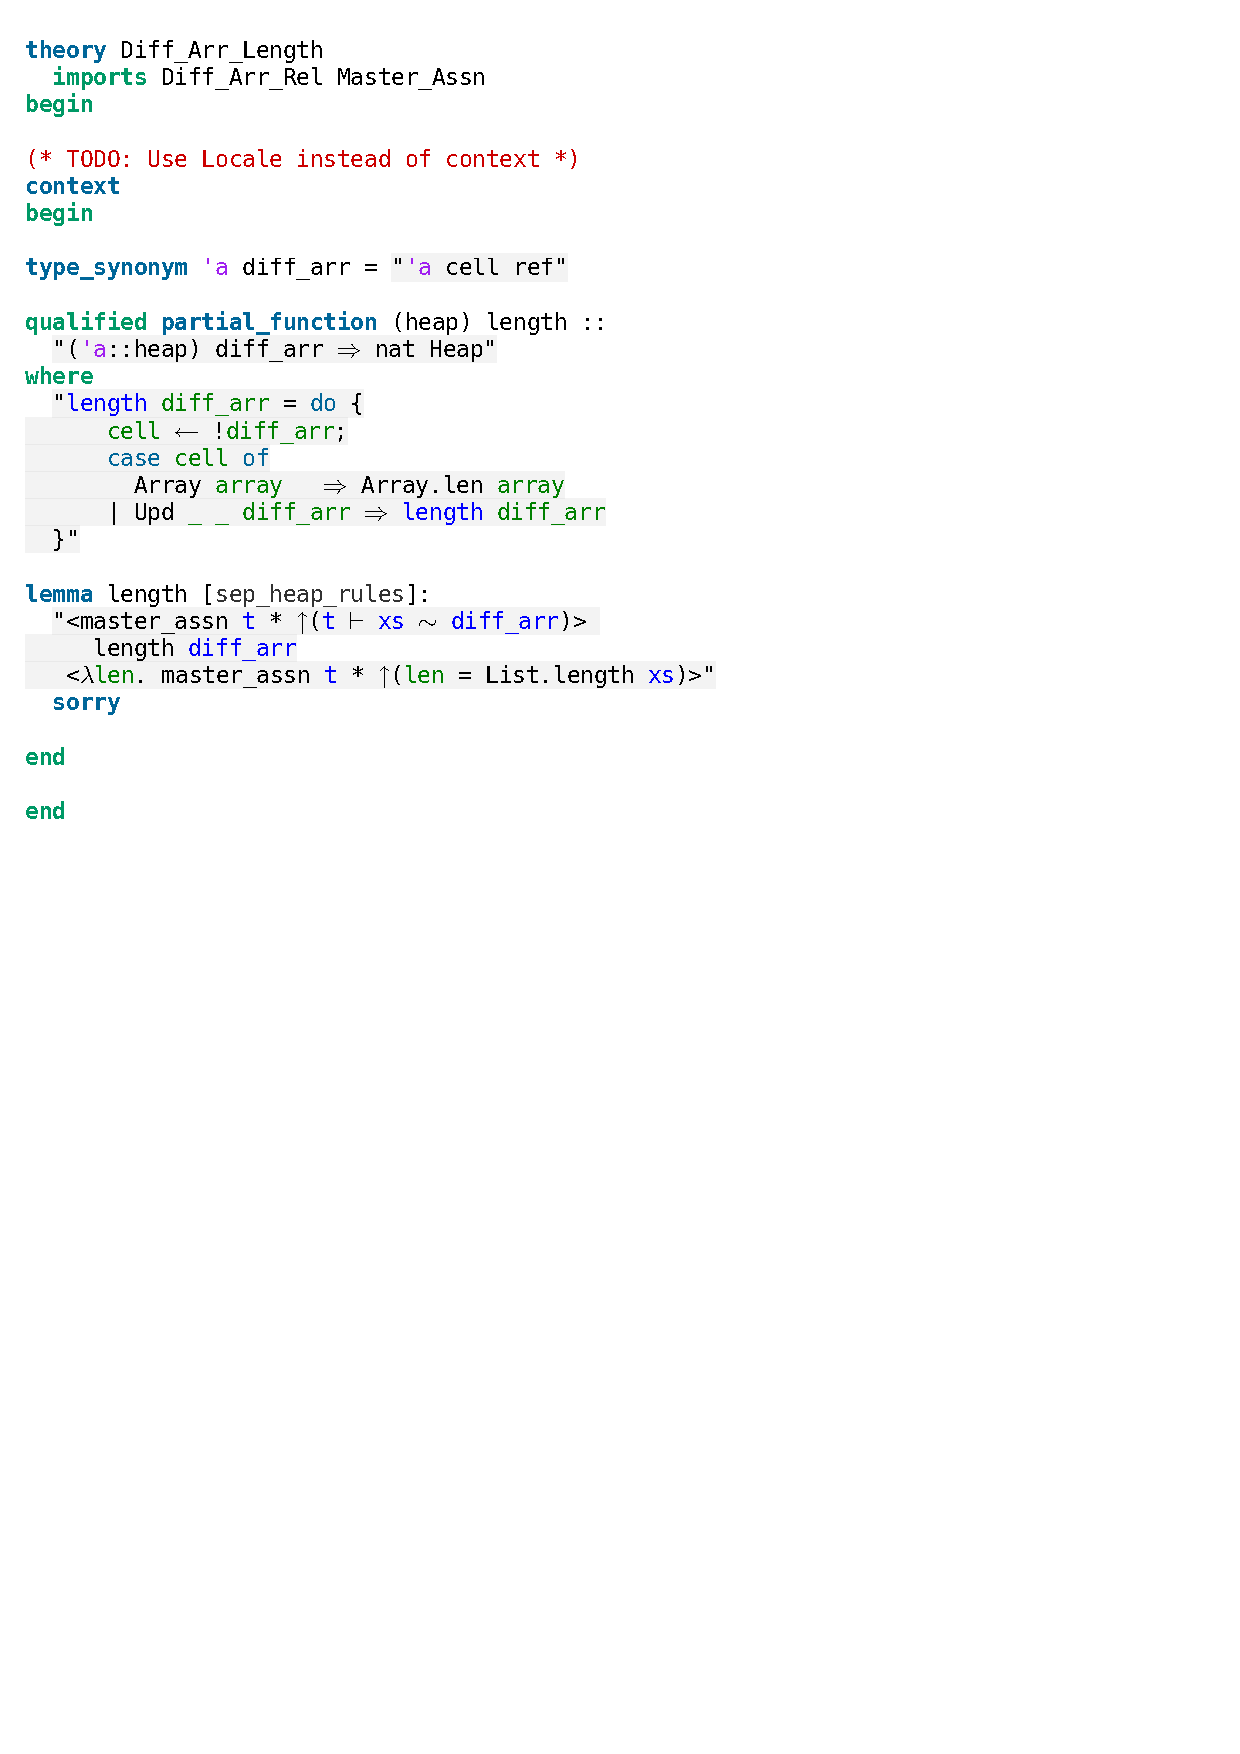
\includegraphics[trim={0 20,2cm 0 5,2cm}, clip, width=1.00\textwidth]{figures/Theory_Diff_Arr_Length.pdf}
    \caption[Diff array length]{Diff array length}
    \label{fig:diff_arr_length}
\end{figure}

\noindent The implementation is straightforward and simply recurses the update chain down to the array cell and returns the length of the plain array\footnote{As a future improvement of the runtime, one could also store the length directly into the cells.}. The proof is similarly straightforward and can be done, for example, by structural induction on the diff array relation of the precondition (\autoref{fig:diff_arr_length_proof}). Both cases of the induction can be proven analogously by first opening and later closing the master assertion, accompanied by the separation logic automation.

\begin{figure}[htpb]
    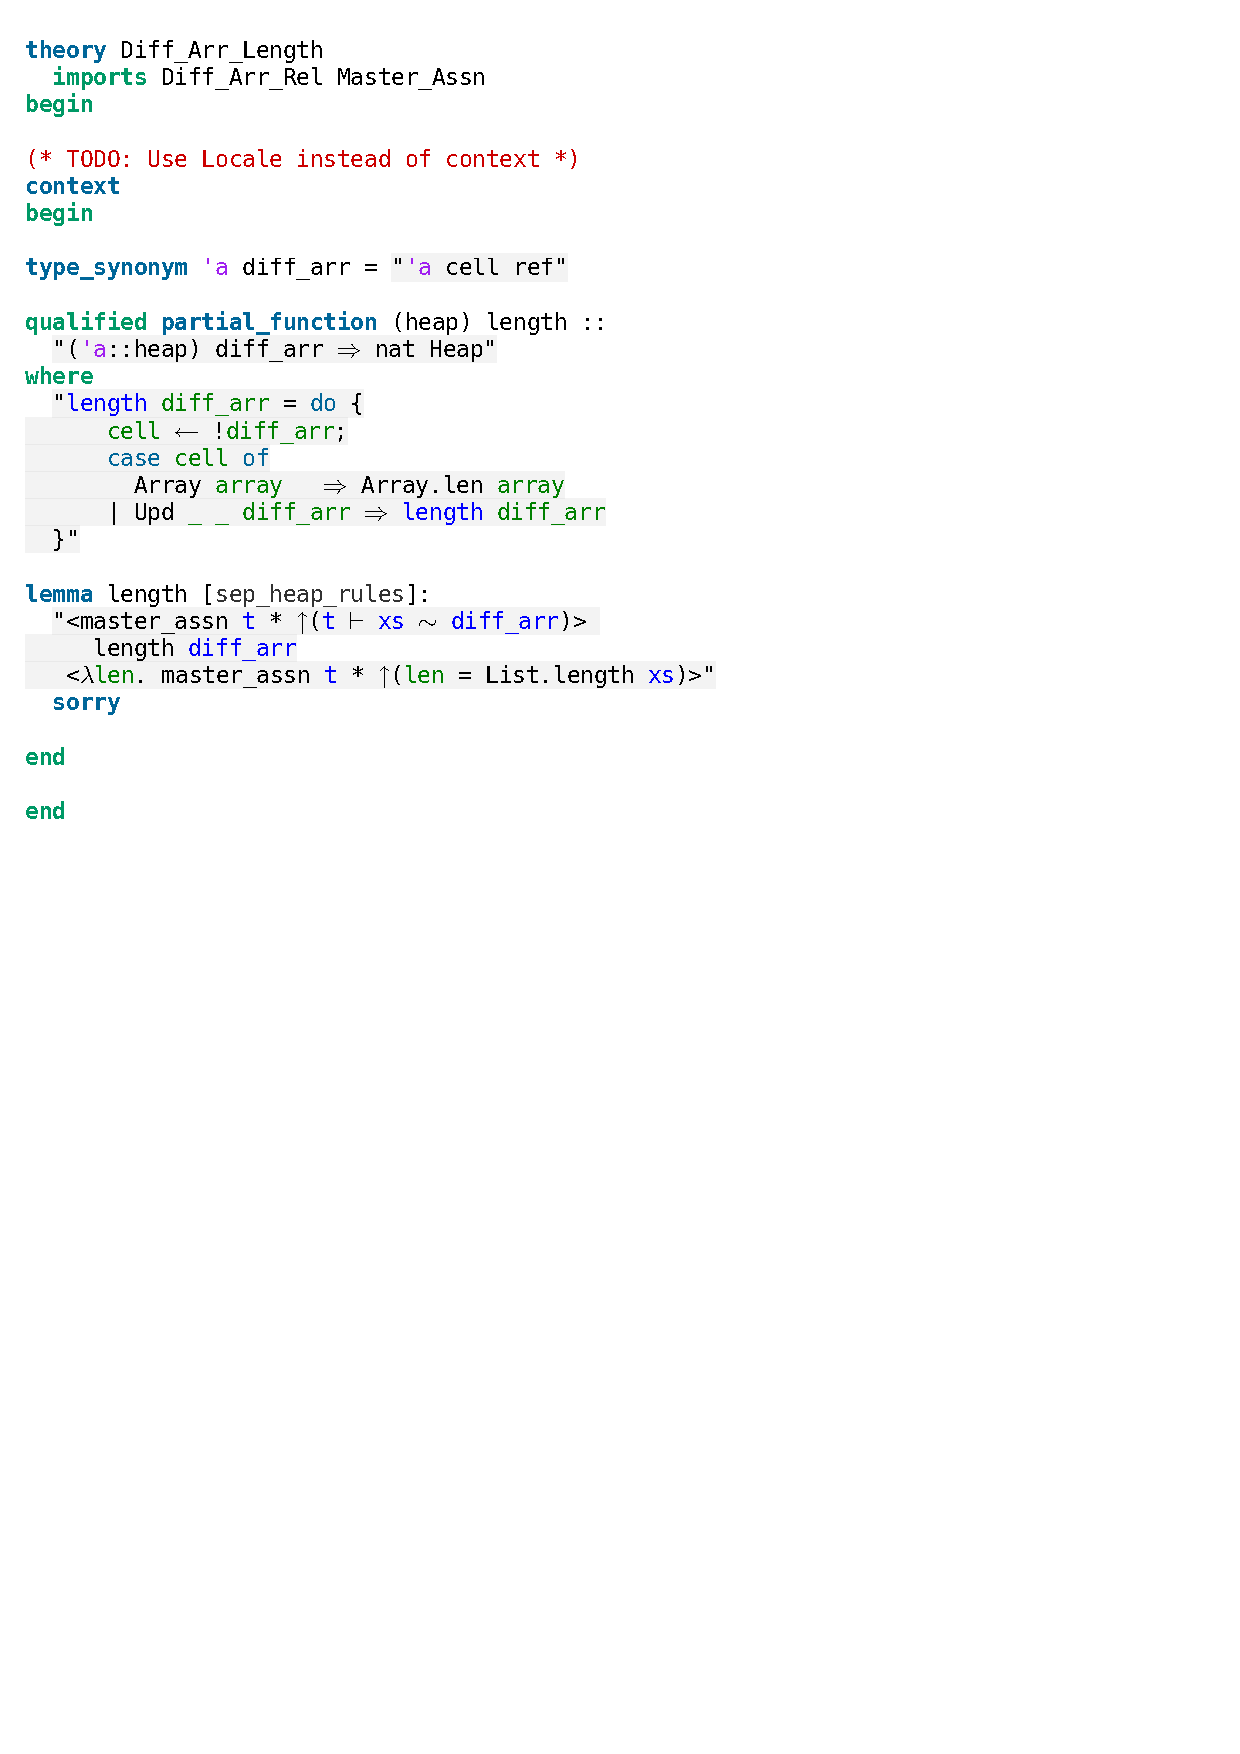
\includegraphics[trim={0 18cm 0 9,8cm}, clip, width=1.00\textwidth]{figures/Theory_Diff_Arr_Length.pdf}
    \caption[Diff array length proof]{Diff array length proof}
    \label{fig:diff_arr_length_proof}
\end{figure}

\subsection{Safe Operations}\label{section:safe_diff_arr}

Before we can go on to automatically replace lists with arrays, we need to simplify one detail of the implementations of the lookup and update operations. The operations expect that the provided index is inside the bounds of the array, and it would be cumbersome just to allow the translation of functions accounting for it.\\
To solve this issue, we define a lookup operation that is undefined for indices out of bounds in a similar way as the standard |List|.|nth| operation (\autoref{fig:diff_arr_lookup_safe}). Like that, the program will exceptionally terminate on an index out of bounds.\\
The update operation does not even need that (\autoref{fig:diff_arr_update_safe}). We simply do not update anything if the index is out of bounds.\\
The proofs for both operations use separation logic proof automation with our previous proofs of the according operations (\autoref{fig:diff_arr_safe_proof}).


\begin{figure}[htpb]
    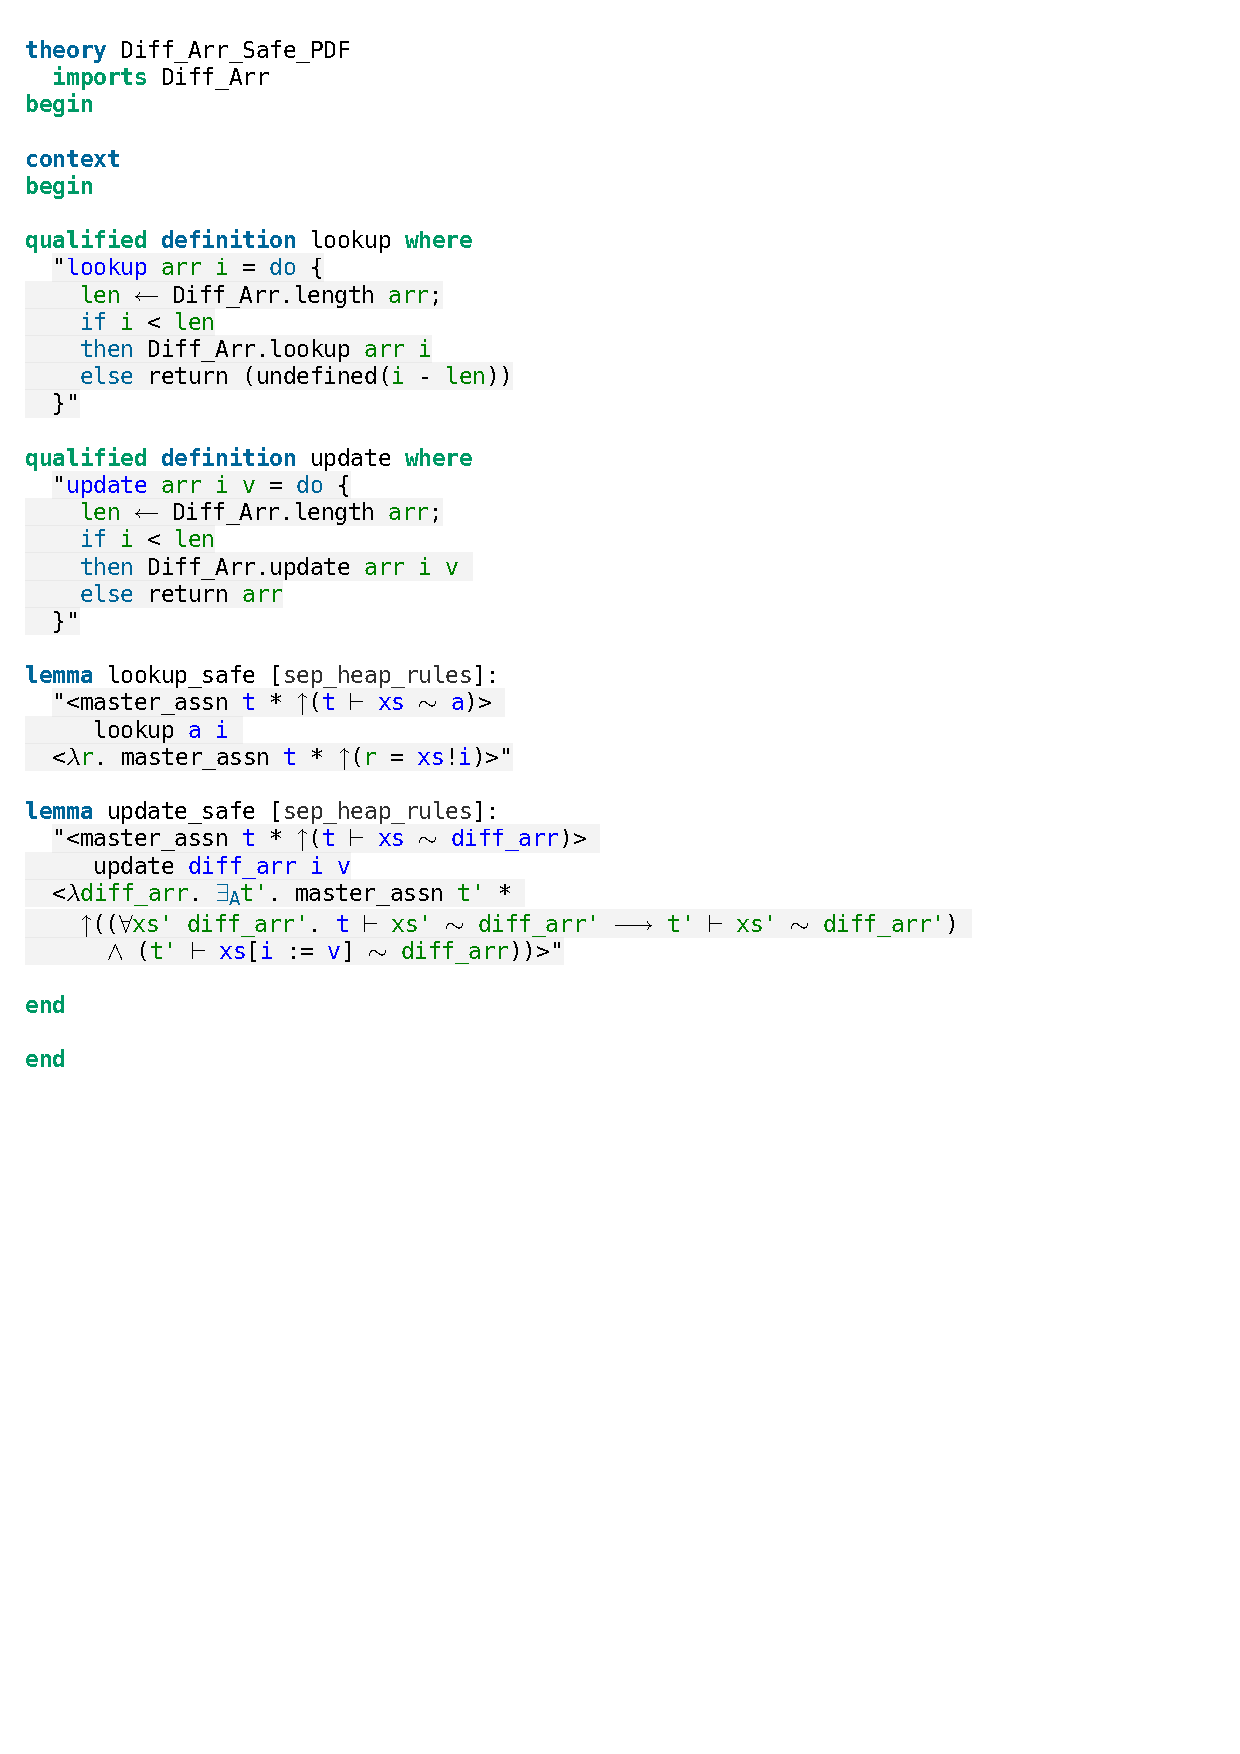
\includegraphics[trim={0 22,6cm 0 3,8cm}, clip, width=1.00\textwidth]{figures/Theory_Diff_Arr_Safe.pdf}
    \caption[Safe diff array lookup]{Safe diff array lookup}
    \label{fig:diff_arr_lookup_safe}
\end{figure}

\begin{figure}[htpb]
    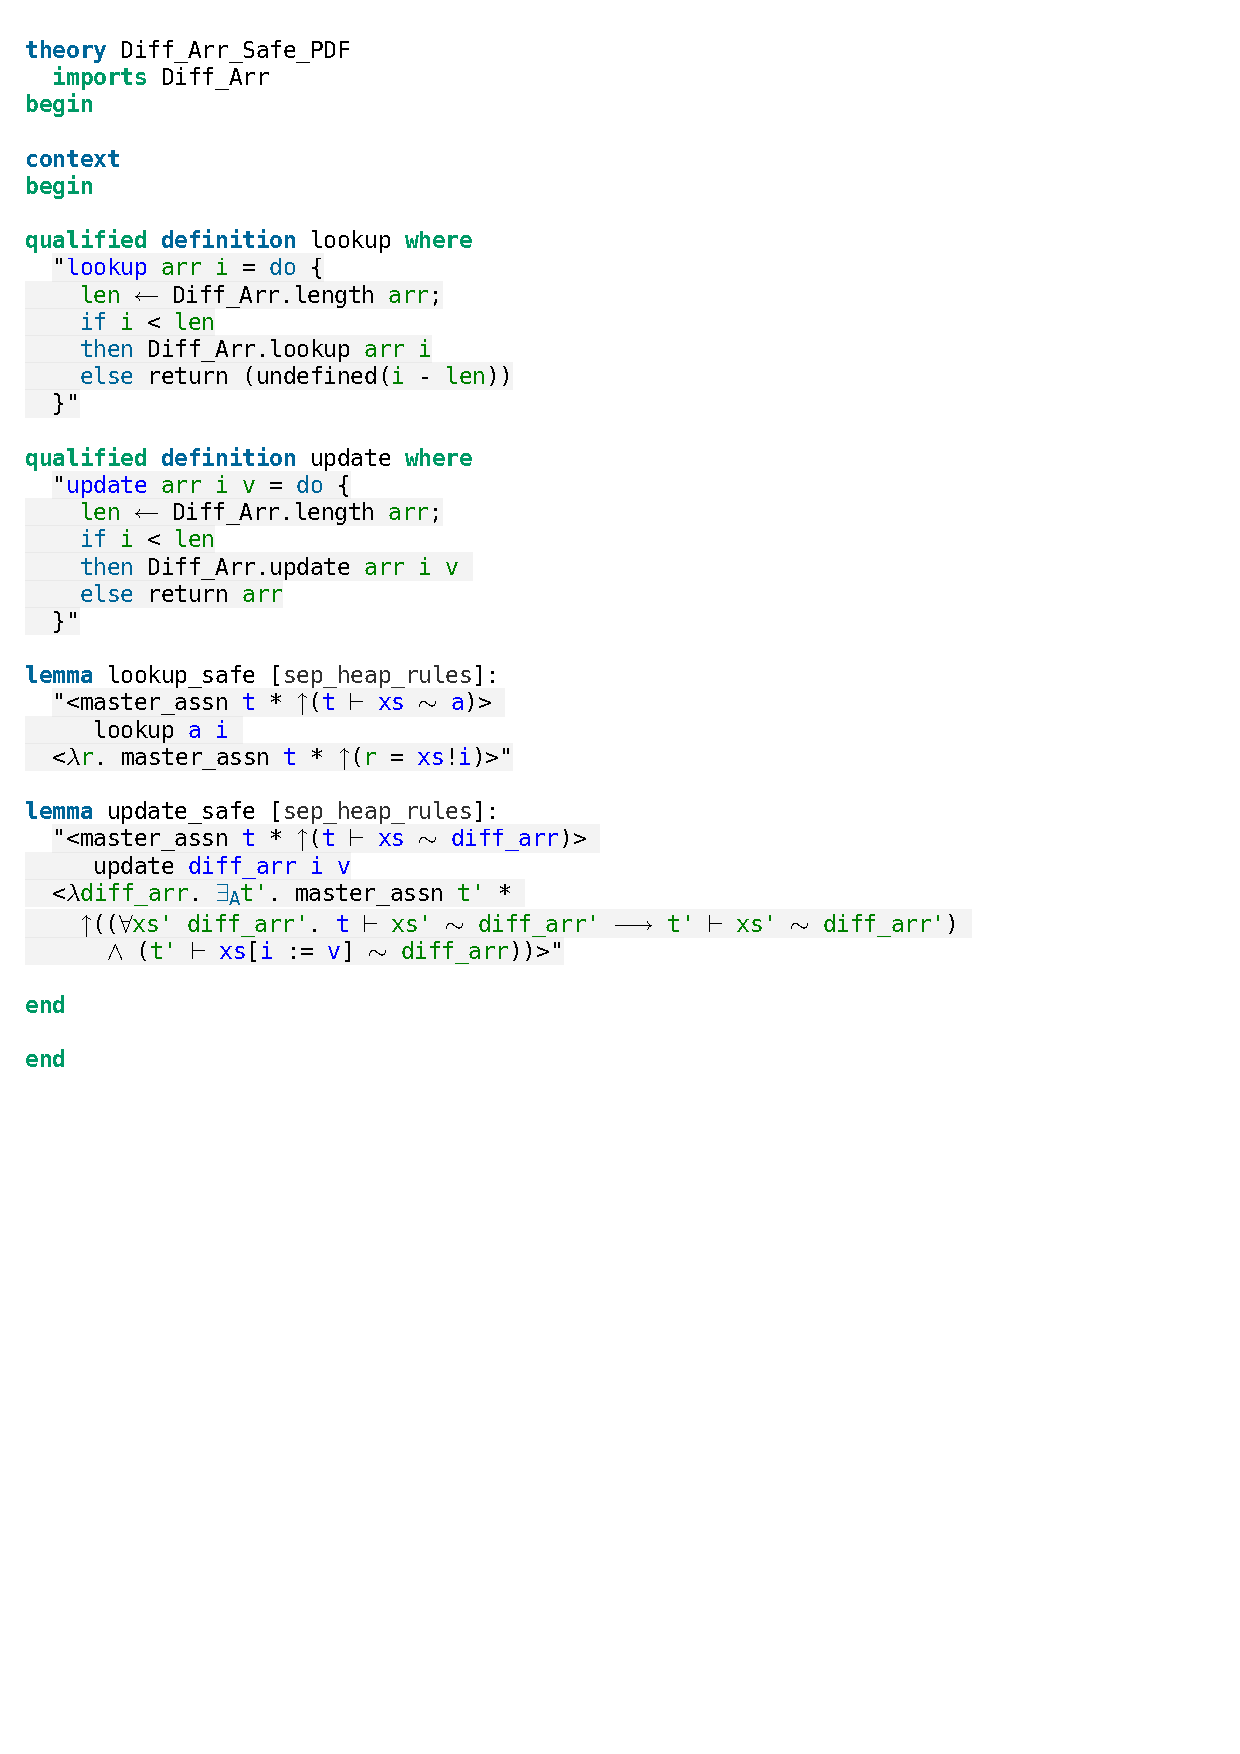
\includegraphics[trim={0 19cm 0 7,6cm}, clip, width=1.00\textwidth]{figures/Theory_Diff_Arr_Safe.pdf}
    \caption[Safe diff array update]{Safe diff array update}
    \label{fig:diff_arr_update_safe}
\end{figure}

\begin{figure}[htpb]
    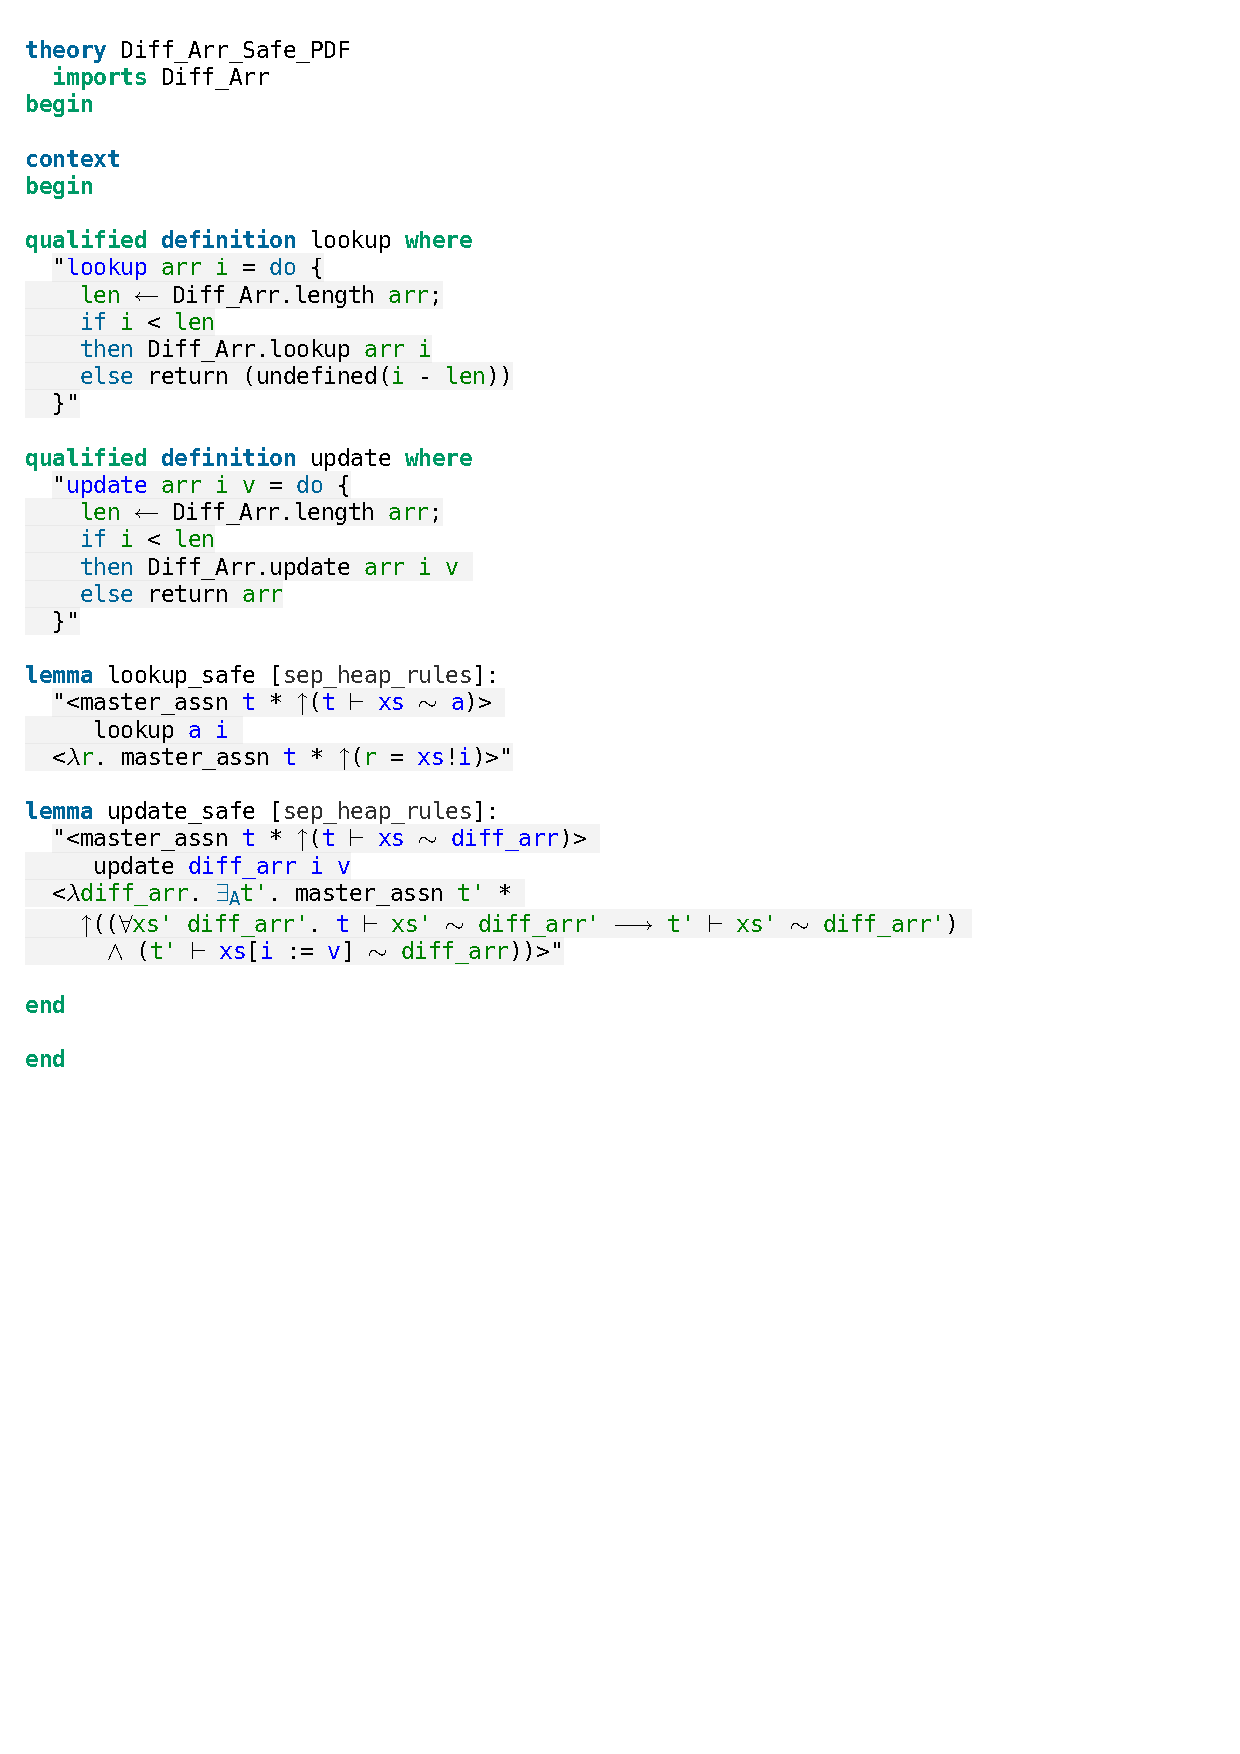
\includegraphics[trim={0 13,4cm 0 11,2cm}, clip, width=1.00\textwidth]{figures/Theory_Diff_Arr_Safe.pdf}
    \caption[Safe diff array operation proofs]{Safe diff array operation proofs}
    \label{fig:diff_arr_safe_proof}
\end{figure}

